
\documentclass[11pt]{article}
\usepackage[letterpaper,margin=0.78in,headheight=15pt]{geometry}
\usepackage[T1]{fontenc}
\usepackage{lmodern}
\usepackage{microtype}
\usepackage{amsmath,amssymb,mathtools}
\usepackage{booktabs,tabularx,longtable,array,multirow}
\usepackage{xcolor}
\usepackage{enumitem}
\usepackage{graphicx}
\usepackage{hyperref}
\usepackage{url}
\usepackage{fancyhdr}
\usepackage[most]{tcolorbox}
\usepackage{listings}
\usepackage{tikz}
\usetikzlibrary{arrows.meta,positioning,shapes.multipart,fit}
\usepackage{pdflscape}
\usepackage{siunitx}
\usepackage{titlesec}
\usepackage{parskip}

\definecolor{navy}{HTML}{17365D}
\definecolor{blue2}{HTML}{2F75B5}
\definecolor{lightblue}{HTML}{EAF3F8}
\definecolor{lightgreen}{HTML}{EDF7ED}
\definecolor{lightgold}{HTML}{FFF6D9}
\definecolor{lightred}{HTML}{FDEDED}
\definecolor{graybg}{HTML}{F4F5F7}
\hypersetup{colorlinks=true,linkcolor=navy,urlcolor=blue2,citecolor=navy}
\pagestyle{fancy}\fancyhf{}
\lhead{MIE 690A - AI in Fluid Mechanics}\rhead{Weeks 5-6 Guided Final Project}\cfoot{\thepage}
\setlist{itemsep=3pt,topsep=4pt,leftmargin=1.5em}
\titleformat{\section}{\Large\bfseries\color{navy}}{\thesection}{0.6em}{}
\titleformat{\subsection}{\large\bfseries\color{blue2}}{\thesubsection}{0.6em}{}
\titleformat{\subsubsection}{\normalsize\bfseries\color{navy}}{\thesubsubsection}{0.6em}{}
\newcolumntype{Y}{>{\raggedright\arraybackslash}X}
\newtcolorbox{summarybox}{colback=lightblue,colframe=blue2,title=Central message,fonttitle=\bfseries,breakable}
\newtcolorbox{definitionbox}[1]{colback=white,colframe=blue2,title=#1,fonttitle=\bfseries,breakable}
\newtcolorbox{projectbox}[1]{colback=lightblue!55,colframe=navy,title=#1,fonttitle=\bfseries,breakable}
\newtcolorbox{deliverbox}{colback=lightgreen,colframe=green!45!black,title=Required deliverable,fonttitle=\bfseries,breakable}
\newtcolorbox{warningbox}{colback=lightgold,colframe=orange!70!black,title=Important boundary,fonttitle=\bfseries,breakable}
\newtcolorbox{failurebox}{colback=lightred,colframe=red!65!black,title=Required failure test,fonttitle=\bfseries,breakable}
\newtcolorbox{prizebox}{colback=lightgold,colframe=navy,title=Project competition and prize pathway,fonttitle=\bfseries,breakable}
\newtcolorbox{codeguide}[1]{colback=graybg,colframe=navy,title=#1,fonttitle=\bfseries,breakable}
\lstset{basicstyle=\ttfamily\small,frame=single,backgroundcolor=\color{graybg},
        breaklines=true,showstringspaces=false,columns=fullflexible,
        keywordstyle=\color{blue2}\bfseries,commentstyle=\color{green!45!black},
        stringstyle=\color{red!65!black},upquote=true}
\urlstyle{tt}
\newcommand{\file}[1]{\path{#1}}
\newcommand{\variant}[1]{\textbf{#1}}

\begin{document}
\begin{titlepage}
\centering
\vspace*{1.0cm}
{\color{navy}\rule{\textwidth}{2pt}}\\[0.45cm]
{\Huge\bfseries Guided Final Projects in\\[0.15cm]AI for Fluid and Kinetic Flows\par}
\vspace{0.35cm}
{\Large Weeks 5-6 Project Guide and Notebook Map (Expanded self-study edition v1.4.2)\par}
\vspace{0.45cm}
{\color{navy}\rule{\textwidth}{2pt}}\\[0.9cm]
{\Large MIE 690A - AI in Fluid Mechanics\par}
\vspace{0.2cm}
{\large Summer 2026\par}
\vfill
\begin{summarybox}
You are not being asked to invent an entire AI-CFD project from nothing. You will begin from a working Week-4 baseline, make one scientifically meaningful extension, and use controlled numerical and physical tests to determine whether that extension is useful.
\end{summarybox}
\vfill
{\large Instructor: Ehsan Roohi\par}
\end{titlepage}

\tableofcontents
\newpage

\section{Executive Summary}
Week 4 taught a common workflow on the lid-driven cavity:
\[
\text{fixed CFD solver}\rightarrow\text{quality-checked fields}\rightarrow
\text{baseline surrogate}\rightarrow\text{field-aware model}\rightarrow\text{validation}.
\]
Weeks 5 and 6 use this common foundation to teach a new skill: \emph{how to design and defend a controlled computational experiment}. Every student selects one of eleven bounded project variants. Track 6 is an instructor-approved research track with substantially more supplied code because it deploys a neural closure inside a particle Fokker--Planck solver. Starter notebooks provide the data loader, baseline model, metrics, and plotting functions. The student owns the split, the one permitted modification, the controlled comparison, the physical interpretation, and the failure analysis.

\begin{warningbox}
Simply rerunning or cosmetically editing a Week-4 notebook is not a final project. Conversely, students are not expected to rewrite the CFD solver, design a research codebase from scratch, or build an unrelated project using automatically generated code.
\end{warningbox}

\subsection{What is new relative to Week 4?}
\begin{tabularx}{\textwidth}{@{}p{0.22\textwidth}YY@{}}
\toprule
& \textbf{Week 4} & \textbf{Weeks 5-6}\\
\midrule
Question & Supplied by the instructor & Selected from one bounded project variant\\
Code & Guided laboratory notebook & Working starter plus designated experiment choices\\
Model & Reproduce and compare supplied baselines & Change one scientifically meaningful element\\
Validation & Follow required metrics & Predeclare criteria, analyze tradeoffs, find failure\\
Conclusion & Explain notebook output & Defend a claim supported by controlled evidence\\
\bottomrule
\end{tabularx}

\section{Learning Objectives}
By the end of the project, a student should be able to:
\begin{enumerate}
\item turn a broad idea into a one-sentence research question;
\item distinguish training, validation, blind test, interpolation, and extrapolation;
\item change one factor at a time and preserve a defensible baseline;
\item evaluate a fluid surrogate with numerical and physical evidence;
\item separate model error from data quality, stochastic variation, and numerical bias;
\item identify a condition where the model is unreliable;
\item explain and modify the important cells in the submitted notebook;
\item document any AI-assisted coding and verify the resulting implementation.
\end{enumerate}

\section{How to Use This Guide}
This document is written as a self-study project manual, not only as a list of deliverables. Each track is organized in four layers:
\begin{enumerate}
\item \textbf{Concept layer:} the physical and machine-learning idea is explained before the code is discussed.
\item \textbf{Provided-code layer:} the notebook cells and helper functions that are already complete are identified.
\item \textbf{Student-decision layer:} the small number of choices that the student is allowed to change are stated explicitly.
\item \textbf{Evidence layer:} the tables, figures, physical checks, and failure test required to support a conclusion are listed.
\end{enumerate}
Students should first run \file{P0_Project_Setup.ipynb}, then read the introductory pages for the selected track, and only then edit the track notebook. The project is intentionally guided: the solver, data loader, most plotting functions, and baseline model are supplied. The independent work is the scientific design, the controlled modification, and the interpretation.

\begin{summarybox}
A student is not expected to understand every helper function before beginning. The student \emph{is} expected to understand the variables being changed, the meaning of the train/validation/test split, the metric used for selection, and the physical meaning of the final plots.
\end{summarybox}

\section{Essential Notation and Definitions}
The same symbols are used throughout the guide and notebooks. This section defines them once so that later equations can be read without guessing.

\subsection{Physical variables for the cavity problem}
\begin{tabularx}{\textwidth}{@{}p{0.14\textwidth}p{0.25\textwidth}Y@{}}
\toprule
\textbf{Symbol} & \textbf{Name} & \textbf{Meaning in this course}\\
\midrule
$L$ & cavity length & Characteristic side length of the square cavity. Coordinates are normalized by $L$, so the computational domain is $0\le x/L\le1$, $0\le y/L\le1$.\\
$U_{\mathrm{lid}}$ & lid speed & Tangential speed of the moving top wall. Velocity is often normalized by this value.\\
$\nu$ & kinematic viscosity & Momentum diffusivity of the continuum fluid.\\
$Re$ & Reynolds number & $Re=U_{\mathrm{lid}}L/\nu$. It measures the ratio of inertial to viscous effects. Increasing $Re$ generally sharpens gradients and changes the vortex structure.\\
$x,y$ & spatial coordinates & Nondimensional coordinates in the cavity. In code, arrays named \texttt{x} and \texttt{y} contain the grid coordinates.\\
$u(x,y),v(x,y)$ & velocity components & Horizontal and vertical velocity components. The moving lid mainly drives positive $u$ near the top wall.\\
$p(x,y)$ & gauge pressure & Pressure recovered from the velocity field and shifted so that its spatial mean is zero. Only pressure differences are physically meaningful in this formulation.\\
$\psi(x,y)$ & streamfunction & A scalar field used in the Week-4 solver. With the convention used in the notebooks, $u=\partial\psi/\partial y$ and $v=-\partial\psi/\partial x$. This automatically gives a divergence-free discrete reference velocity field.\\
$\omega(x,y)$ & vorticity & In two dimensions, $\omega=\partial v/\partial x-\partial u/\partial y$. It measures local rotation of the flow.\\
$\lambda$ & mean free path & Average molecular distance between collisions in the kinetic/rarefied track.\\
$Kn$ & Knudsen number & $Kn=\lambda/L$. It measures rarefaction. Small $Kn$ is continuum-like; larger $Kn$ requires kinetic descriptions.\\
\bottomrule
\end{tabularx}

\subsection{Grid, field, and case notation}
A \textbf{grid point} is one spatial location $(x_j,y_j)$. A \textbf{field} is the value of a variable at every grid point, for example the full $u$ array at one Reynolds number. A \textbf{case} is one complete physical simulation condition, such as one full cavity solution at $Re=275$ or one stochastic kinetic run at a specified $(Kn,U_{\mathrm{wall}},\text{seed})$.

Let $N_x$ and $N_y$ be the number of grid points in the two directions and let
\[
N_g=N_xN_y
\]
be the number of spatial points in one scalar field. In the supplied continuum dataset, $N_x=N_y=65$, so $N_g=4225$. A three-output field $(u,v,p)$ therefore contains $3N_g=12675$ scalar values per physical case.

\begin{warningbox}
Grid points from the same case are not independent physical simulations. Randomly sending some points from one case to training and other points from the same case to testing creates leakage. The project notebooks split complete cases, not random points.
\end{warningbox}

\subsection{Machine-learning notation}
\begin{tabularx}{\textwidth}{@{}p{0.16\textwidth}p{0.25\textwidth}Y@{}}
\toprule
\textbf{Symbol} & \textbf{Name} & \textbf{Meaning}\\
\midrule
$\mathbf z$ & model input & Input vector supplied to a network. For a coordinate DNN, $\mathbf z=(Re,x,y)$. For Track 5, $\mathbf z=(\log_{10}Kn,U_{\mathrm{wall}},x,y)$.\\
$\mathbf y$ & target/label & Reference output used for training, for example $(u,v,p)$. The label may contain numerical error or stochastic noise.\\
$\widehat{\mathbf y}$ & prediction & Model output. A hat always denotes a predicted or reconstructed quantity.\\
$f_{\theta}$ & neural model & Function represented by a neural network. $\theta$ denotes all trainable weights and biases.\\
$\mathcal L_{\mathrm{data}}$ & data loss & Error between prediction and label, usually mean squared error.\\
$\mathcal L_{\mathrm{phys}}$ & physics loss & Additional penalty based on a physical property, such as divergence or a boundary condition.\\
$\lambda_{\mathrm{phys}}$ & physics weight & Nonnegative coefficient controlling the strength of the physics penalty relative to the data loss.\\
$\mu_j,s_j$ & scaler statistics & Mean and standard deviation of feature $j$, computed from training data only.\\
$r$ & reduced rank & Number of POD modes retained in a reduced representation.\\
$\phi_k$ & POD mode & The $k$th spatial basis function. It is a field-shaped pattern learned from development snapshots.\\
$a_k$ & modal coefficient & Scalar amplitude multiplying POD mode $\phi_k$ for a particular physical case.\\
$\sigma_k$ & singular value & Strength of POD mode $k$ in the snapshot dataset.\\
\bottomrule
\end{tabularx}

\subsection{Additional notation for the Fokker--Planck closure track}
Track 6 does not predict a final flow field directly. It learns the expensive local closure map used inside a particle Fokker--Planck solver. The symbols below are introduced here because they are different from the coordinate-DNN notation used in Tracks 1--5.

\begin{tabularx}{\textwidth}{@{}p{0.17\textwidth}p{0.25\textwidth}Y@{}}
\toprule
\textbf{Symbol} & \textbf{Name} & \textbf{Meaning in Track 6}\\
\midrule
$\rho$ & mass density & Cell mass density obtained from particle weights divided by cell volume.\\
$T$ & translational temperature & Temperature obtained from the second central moment of molecular velocity.\\
$U_i$ & bulk velocity & Cell-average molecular velocity in direction $i$.\\
$\Pi_{ij}$ & second central moment / pressure tensor input & Six independent symmetric components used by the neural closure. In the supplied code the array is named \texttt{PIJ}.\\
$q_i$ & heat-flux moment input & Three third-order central-moment components; the code stores them in \texttt{Q}.\\
$DM2$ & scalar second central moment & $DM2=\langle c_i c_i\rangle$, where $\mathbf c=\mathbf V-\mathbf U$ is peculiar velocity. It is proportional to temperature.\\
$\nu$ & relaxation/collision-frequency feature & Local scalar frequency available to both the exact and learned closure paths.\\
$C_{ij}$ & stress-relaxation coefficients & Six symmetric coefficients of the cubic-FP drift. The code stores them in the first six output channels and in \texttt{coeffs['A']}.\\
$\Gamma_i$ & heat-flux relaxation coefficients & Three coefficients controlling the heat-flux part of the drift. The code stores them in the last three output channels and in \texttt{coeffs['B']}.\\
$\mathbf x_{FP}$ & closure-network input & The 16-component vector $(\rho,T,U_i,\Pi_{ij},q_i,DM2,\nu)$.\\
$\mathbf y_{FP}$ & exact closure target & The 9-component vector $(C_{ij},\Gamma_i)$ returned by the high-order moment assembly and exact local $9\times9$ solve.\\
\bottomrule
\end{tabularx}

A small coefficient-regression error is not the final objective. The trained coefficients are inserted back into the stochastic particle update, so Track 6 also requires a complete \emph{closed-loop} cavity test. This distinguishes an offline regression benchmark from an operational physics--ML solver.

\subsection{Training, validation, development, and blind test}
The terms below have different purposes and must not be interchanged.
\begin{itemize}
\item \textbf{Training cases} update the network parameters $\theta$.
\item \textbf{Validation cases} are not used in gradient updates. They are used to select architecture, rank, loss weight, or stopping epoch.
\item \textbf{Development set} means the training plus validation cases that are permitted during model design. After the design is frozen, the final model may be retrained using all permitted development cases.
\item \textbf{Blind test cases} remain closed until all design choices are fixed. They estimate generalization to unseen physical cases.
\end{itemize}

A model is not truly blind-tested if the student changes architecture, rank, loss weight, or stopping rule after viewing the test result.

\section{Core Concepts Used in Every Track}
\subsection{Full-order reference model and surrogate model}
The Week-4 cavity solver is the \textbf{full-order reference model} for this project. It numerically solves the governing equations on a fixed grid and produces complete fields. A \textbf{surrogate model} is a cheaper approximation trained to reproduce the reference solution over a family of inputs.

The surrogate does not replace the physical equations in a universal sense. It approximates the mapping represented by the available dataset. If the reference solver contains grid error, pressure-recovery error, or limited accuracy at high $Re$, the surrogate learns those labels. Therefore, ``small error against the dataset'' and ``physical truth'' are not identical claims.

\subsection{Coordinate DNN: turning fields into supervised samples}
The coordinate network used in Week 4 learns
\[
\widehat{\mathbf y}=f_{\theta}(Re,x,y),
\qquad
\widehat{\mathbf y}=(\hat u,\hat v,\hat p).
\]
For every development Reynolds number, each grid point becomes one supervised row. The same network represents the entire field because spatial coordinates are part of the input.

Before training, each input feature is standardized using training statistics:
\[
z_j^{\mathrm{scaled}}=\frac{z_j-\mu_j}{s_j}.
\]
Each output channel is also standardized so that $u$, $v$, and $p$ contribute comparably to the loss. The scalers must be fitted on the training cases only; otherwise validation or test information leaks into training.

The baseline data loss is
\[
\mathcal L_{\mathrm{data}}
=\frac{1}{N_b}\sum_{i=1}^{N_b}
\left\|\widehat{\mathbf y}_i-\mathbf y_i\right\|_2^2,
\]
where $N_b$ is the number of point samples in a mini-batch. Minimizing this quantity improves average pointwise agreement, but it does not guarantee correct wall behavior, zero divergence, accurate vortex location, or reliable extrapolation.

\subsection{Interpolation and extrapolation}
\textbf{Interpolation} predicts inside the range covered by development cases. For example, training at $Re=250$ and $Re=300$ and testing at $Re=275$ is interpolation. \textbf{Extrapolation} predicts outside the covered range, such as training only up to $Re=300$ and testing at $Re=400$.

Interpolation can still fail locally, especially near walls or weak secondary vortices. Extrapolation can look visually smooth while being quantitatively wrong. Therefore, both must be checked with reference fields, centerlines, and physical metrics.

\subsection{Numerical error versus physical error}
A global relative $L_2$ error measures average field disagreement. A physical check asks whether the prediction respects a property that matters for the flow. These two kinds of evidence answer different questions.

For example, a model may have a small global velocity error but a large wall error because most grid points are in the interior. Conversely, a strong divergence penalty may reduce divergence while slightly increasing velocity error. The project should report the tradeoff rather than hiding one metric.

\subsection{Controlled experiment}
A controlled experiment changes one primary factor while keeping the comparison fair. The baseline and modified model should use the same development cases, blind cases, output normalization, architecture where possible, optimizer, seed policy, and metric definitions. The purpose is to attribute the observed change to the intended modification.

\begin{definitionbox}{What counts as a scientific conclusion?}
A conclusion is a bounded statement supported by the experiment, for example: ``Within $100\le Re\le300$, direct field interpolation was more accurate than the tested coordinate DNN, while the DNN produced smoother but less accurate high-$Re$ centerlines.'' A statement such as ``neural networks are good for CFD'' is too broad for the evidence.
\end{definitionbox}


\section{The Guided Project Workflow}
\begin{center}
\resizebox{\textwidth}{!}{%
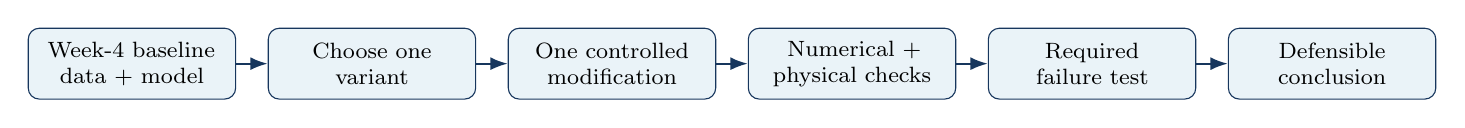
\begin{tikzpicture}[node distance=6mm and 4mm, every node/.style={font=\footnotesize},
box/.style={draw=navy,rounded corners,fill=lightblue,minimum height=9mm,text width=24mm,align=center},
arrow/.style={-{Latex[length=2.2mm]},thick,draw=navy}]
\node[box] (w4) {Week-4 baseline\\data + model};
\node[box,right=of w4] (choice) {Choose one\\variant};
\node[box,right=of choice] (mod) {One controlled\\modification};
\node[box,right=of mod] (phys) {Numerical +\\physical checks};
\node[box,right=of phys] (fail) {Required\\failure test};
\node[box,right=of fail] (claim) {Defensible\\conclusion};
\draw[arrow] (w4)--(choice);\draw[arrow](choice)--(mod);\draw[arrow](mod)--(phys);
\draw[arrow](phys)--(fail);\draw[arrow](fail)--(claim);
\end{tikzpicture}%
}
\end{center}

\subsection{Six tracks, eleven project variants}
\begin{tabularx}{\textwidth}{@{}p{0.10\textwidth}p{0.25\textwidth}YY@{}}
\toprule
\textbf{Variant} & \textbf{Track} & \textbf{Scientific question} & \textbf{Level}\\
\midrule
1A & Reynolds generalization & Interpolation at unseen Reynolds numbers & Intermediate\\
1B & Reynolds generalization & Higher-Re extrapolation and failure boundary & Intermediate\\
2A & Physics-guided DNN & Does wall-weighted learning improve wall accuracy? & Intermediate\\
2B & Physics-guided DNN & Does divergence regularization improve incompressibility? & Advanced\\
3A & POD study & What is the smallest useful POD rank? & Intermediate\\
3B & POD study & Separate output bases or one shared scaled basis? & Intermediate/Advanced\\
4A & Uncertainty & How variable are repeated neural-network trainings? & Intermediate\\
4B & Data sufficiency & How many physical Reynolds-number cases are needed? & Intermediate\\
5A & Rarefied cavity & Do seed-averaged DSMC labels improve the surrogate? & Advanced\\
5B & Rarefied cavity & Can a model generalize to an unseen higher Kn? & Advanced\\
6A & Fokker--Planck neural closure & Can a q-weighted 16-to-9 closure surrogate retain held-out cavity fidelity when deployed inside the particle solver? & Advanced research / instructor approval\\
\bottomrule
\end{tabularx}

\subsection{Project competition, prizes, and prize-track variants}
\begin{prizebox}
At the end of the term, the instructor will award prizes for the top three final projects:
\textbf{First Prize: \$500}, \textbf{Second Prize: \$300}, and \textbf{Third Prize: \$200}.
A project may earn a high course grade without being competitive for a prize. Prize consideration is reserved for work with a realistic pathway to a \textbf{conference-quality submission} and, in the strongest cases, a \textbf{journal-quality continuation} if the student chooses to extend the study.
\end{prizebox}

All eleven variants can receive full course credit. The variants below are the most natural \emph{prize-track candidates} because they support a sharper research claim, a matched representation benchmark, or a direct continuation toward fluid/kinetic research.

\begin{tabularx}{\textwidth}{@{}p{0.10\textwidth}Y@{}}
\toprule
\textbf{Variant} & \textbf{Why it is a natural prize-track candidate}\\
\midrule
1B & A clear extrapolation and failure-boundary study can produce a defensible conference claim if the trustworthy and breakdown regimes are identified with matched baselines and physical evidence.\\
2B & A physics-guided loss can support a meaningful claim if divergence improves without unacceptable global-error degradation and the result is supported by a controlled ablation.\\
3A & POD-rank sensitivity directly studies compression, field fidelity, runtime/storage, and the loss of local physical structures. This is closely aligned with compact-representation research.\\
3B & Separate versus shared bases can become a matched-capacity representation study, especially if the student explains why a common basis succeeds or fails for velocity and pressure.\\
5A & Noise-aware learning from repeated kinetic simulations can separate surrogate error from sampling variability and is a strong basis for a rarefied-flow conference study.\\
5B & Generalization across Knudsen number can expose regime transfer and failure; with stronger reference data and extended validation it has a plausible journal continuation path.\\
6A & The project mirrors an active GPU-native Fokker--Planck closure study and combines data generation, q-weighted learning, native deployment, complete-condition testing, high-order diagnostics, and runtime analysis. It is the strongest direct conference/journal continuation track when executed at production resolution.\\
\bottomrule
\end{tabularx}

Projects inspired by \emph{compact, physically faithful representations} are especially encouraged for the prize track. This means using matched-storage or matched-capacity baselines where appropriate, preserving quantities that matter physically rather than only smooth low-order fields, and making a claim about fidelity, compression, uncertainty, or regime transfer that remains meaningful beyond this course.

\subsection{Minimum standard for prize consideration}
A prize candidate must satisfy all normal course requirements and also reach the higher standard below.
\begin{enumerate}
\item \textbf{Clear research question.} The question is narrow, testable, and physically meaningful.
\item \textbf{Substantive extension beyond Week 4.} Changing only a plot, seed, or split is insufficient. The project adds a physics-guided objective, representation benchmark, uncertainty/noise study, or regime-transfer experiment.
\item \textbf{Matched baseline comparison.} The baseline and modification use the same permitted data, metric definitions, and as many identical training choices as possible.
\item \textbf{Multiple forms of evidence.} Report numerical metrics and at least \textbf{three} physical checks; at least one must be local or structure-aware, such as wall behavior, vortex location, pressure centerlines, divergence, recirculation topology, or a moment-sensitive quantity.
\item \textbf{Ablation or sensitivity study.} Include at least one controlled parameter sweep, rank study, penalty study, case-count study, or matched-capacity comparison.
\item \textbf{Failure analysis.} Show a condition where the model becomes inaccurate or physically unreliable and explain the mechanism.
\item \textbf{Reproducibility.} The submitted notebook runs top-to-bottom with all required files and records the final configuration, seeds, versions, and data hash.
\item \textbf{Research-quality communication.} Figures are publication-style, and the report includes an abstract-style summary and a conclusion that states what was learned.
\end{enumerate}

\subsection{Conference-level and journal-path expectations}
A project is \textbf{conference-level} when it makes one clean technical claim with adequate evidence, a matched baseline, and an honest scope/limitation statement. A project has a plausible \textbf{journal-path continuation} when the class result opens a broader question that can be extended with additional cases, stronger reference data, deeper validation, or a more capable method. The six-week project is not expected to become a paper immediately; the goal is for the strongest projects to become credible seeds for a conference abstract or later manuscript.

\subsection{Optional stretch extensions for advanced students}
The required project defines the common floor. Students who complete the required comparison early may request approval for \textbf{one} optional stretch extension listed under the selected track. Stretch work is not required for full course credit and should not be started until the Week-5 checkpoint is complete. Its purpose is to raise the ceiling for strong doctoral students and prize-track projects without increasing the entry barrier for the class. A stretch extension should add one new scientific dimension while preserving the original matched baseline and blind-test discipline.

\section{What the Instructor Provides and What the Student Owns}
\subsection{Provided material}
\begin{itemize}
\item a fixed Week-4 cavity dataset and quality-control protocol;
\item a common file-check notebook, \file{P0_Project_Setup.ipynb};
\item one starter notebook for each project track;
\item reusable loading, training, metric, POD, plotting, and mini-DSMC functions;
\item for Track 6, a supplied particle-FP reference solver, exact-data generator, TensorFlow trainer, CuPy deployment wrapper, and closed-loop analyzer;
\item a bounded set of model choices and experiment variables;
\item required metrics, physical checks, and report templates.
\end{itemize}

\subsection{Student responsibility}
\begin{itemize}
\item choose one variant and state one research question;
\item run and explain the supplied baseline;
\item freeze the split and comparison plan before blind testing;
\item make the required modification and no uncontrolled simultaneous changes;
\item generate a reproducible table and three to five decision-relevant figures;
\item perform at least two physical checks;
\item identify and explain one failure or tradeoff;
\item defend one important code cell and one scientific conclusion.
\end{itemize}

\begin{summarybox}
The project is not graded by the number of lines of new code. It is graded by the quality of the experiment, the validity of the comparison, the physical reasoning, and the student's ability to explain the implementation.
\end{summarybox}

\section{Minimum Viable Project}
Every approved project must contain all eight items below.
\begin{enumerate}
\item A reproduced baseline from the supplied notebook.
\item One extension beyond Week 4.
\item A controlled baseline-versus-modification comparison.
\item A case-wise train/validation/test design.
\item At least two physical-validation checks.
\item One documented failure condition or tradeoff.
\item One metric table and three to five useful figures.
\item A short code-origin statement and a five-minute code defense.
\end{enumerate}

\begin{deliverbox}
A project that produces a lower loss but does not include physical checks and a failure analysis is incomplete. A project whose modification does not outperform the baseline may still receive full credit if the experiment is correct and the negative result is explained honestly.
\end{deliverbox}

\section{Project Timeline}
\subsection{Beginning of Week 5: setup submission}
Run \file{P0_Project_Setup.ipynb} and submit:
\begin{itemize}
\item \file{project_choice.json};
\item the dataset audit;
\item the Re=275 interpolation baseline table;
\item the selected track notebook filename.
\end{itemize}

\subsection{End of Week 5: mandatory checkpoint}
Submit one ZIP containing:
\begin{enumerate}
\item an executable notebook with the baseline reproduced;
\item a frozen configuration/split cell;
\item one preliminary modified result;
\item one numerical comparison table;
\item one physical check;
\item a paragraph naming the planned failure test;
\item an AI/code-assistance log, even if the entry is ``none.''
\end{enumerate}

\subsection{End of Week 6: final project}
Submit:
\begin{itemize}
\item one clean executed notebook;
\item one PDF report of approximately 6--10 pages;
\item all CSV/NPZ files needed to reproduce reported figures;
\item \file{reproducibility.txt} with seed, package versions, runtime, and hardware;
\item a 5--7 minute presentation or code/results discussion, as assigned.
\end{itemize}

\section{File Organization and Colab Workflow}
Use short filenames and one flat working folder in Colab.
\begin{lstlisting}[language=bash]
project_folder/
  P0_Project_Setup.ipynb
  P2_Physics_Guided_DNN.ipynb   # example selected notebook
  w4utils.py
  w5_common.py
  cavity_data.npz
  project_choice.json
  P2_results.csv
\end{lstlisting}
Track 5 additionally requires \file{mini_dsmc.py}. Track 6 uses the supplied \file{Track6_FP_Cavity} files and should be unpacked as one flat folder on a GPU runtime. Do not upload unrelated Colab sample datasets such as MNIST or California Housing.

To reduce Windows path-length problems and Colab upload friction, the instructor also provides one \textbf{flat ZIP} for setup and one for each track: \file{P0_Setup_v1_4_2.zip}, \file{Track1_Re_v1_4_2.zip}, \file{Track2_Physics_v1_4_2.zip}, \file{Track3_POD_v1_4_2.zip}, \file{Track4_Uncertainty_v1_4_2.zip}, \file{Track5_Kinetic_v1_4_2.zip}, and \file{Track6_FP_Closure_v1_4_2.zip}. Each track ZIP includes the required notebook and helper/data files; the Track-6 ZIP contains the separate FP reference solver and wrappers rather than the Week-4 continuum dataset.

\section{Common Numerical and Physical Evidence}
Every track uses the same philosophy: one scalar score is not enough. The final claim should be supported by global numerical error, local profile evidence, and physical checks related to the chosen research question.

\subsection{Global relative velocity error}
For a blind field on all grid points,
\[
E_{uv}=
\frac{
\sqrt{\sum_{j=1}^{N_g}
[(\hat u_j-u_j)^2+(\hat v_j-v_j)^2]}}
{
\sqrt{\sum_{j=1}^{N_g}(u_j^2+v_j^2)}+\varepsilon
},
\]
where $j$ indexes grid points and $\varepsilon$ is a very small number preventing division by zero. The numerator is the $L_2$ norm of the vector-velocity error; the denominator is the $L_2$ norm of the reference velocity.

This metric measures average field fidelity relative to the overall velocity magnitude. It can be dominated by the primary vortex and may underweight weak corner structures.

\subsection{Pressure error and pressure gauge}
Pressure is stored as zero-mean gauge pressure:
\[
\frac{1}{N_g}\sum_{j=1}^{N_g}p_j=0.
\]
The global relative pressure error is
\[
E_p=\frac{\|\hat p-p\|_2}{\|p\|_2+\varepsilon}.
\]
Because recovered pressure is especially sensitive near the discontinuous lid corners, the notebooks also report an \textbf{interior pressure error} after removing a thin boundary rim. This allows the student to distinguish interior field fidelity from corner sensitivity.

\subsection{Mean absolute error and percentile error}
For a scalar field $q$,
\[
\mathrm{MAE}(q)=\frac{1}{N_g}\sum_{j=1}^{N_g}|\hat q_j-q_j|.
\]
For vector velocity, the pointwise vector error is
\[
e_j^{\mathrm{vec}}=
\sqrt{(\hat u_j-u_j)^2+(\hat v_j-v_j)^2}.
\]
The 95th percentile of $e_j^{\mathrm{vec}}$ describes a high but not single-point-dominated error level. It is often more informative than the maximum error, which may be controlled by one corner node.

\subsection{Centerline errors}
Two standard cavity diagnostics are:
\begin{itemize}
\item vertical profile $u(x/L=0.5,y/L)$;
\item horizontal profile $v(x/L,y/L=0.5)$.
\end{itemize}
A relative centerline error is computed using the same $L_2$ idea but only on profile points. Centerlines are valuable because two streamline plots may look similar even when the velocity distribution through the vortex is different.

\subsection{Wall metrics}
The stationary walls require no penetration and no slip in the continuum reference, while the top wall has $u=U_{\mathrm{lid}}$ away from the corners. The project wall metric combines wall velocity residuals. The four corner nodes are excluded because the moving-lid and stationary-wall conditions meet discontinuously there. With this convention, the CFD reference itself has zero wall error.

Students should report both a wall RMS metric and a lid-specific mean absolute error when wall behavior is relevant.

\subsection{Divergence metric}
For an incompressible prediction,
\[
D(x,y)=\frac{\partial \hat u}{\partial x}
+\frac{\partial \hat v}{\partial y}.
\]
The notebooks report norms such as
\[
D_{L_2}=
\sqrt{\frac{1}{N_g}\sum_{j=1}^{N_g}D_j^2},
\qquad
D_{L_\infty}=\max_j|D_j|.
\]
The reference velocity obtained from the discrete streamfunction is divergence-free to machine precision under the corresponding central-difference operators. A DNN trained only on pointwise data generally is not.

\subsection{Vortex and recirculation evidence}
A cavity field should be checked for the direction and location of the primary recirculation. Possible diagnostics include:
\begin{itemize}
\item sign of the lower-cavity return flow;
\item approximate primary-vortex center;
\item presence or loss of weak corner/secondary recirculation;
\item streamline topology and consistency with centerlines.
\end{itemize}
These checks are often qualitative plus quantitative. A project should avoid claiming a precise vortex location when the reference grid or stochastic field does not support that precision.

\subsection{How to choose physical checks}
Choose checks that directly test the project claim.
\begin{itemize}
\item Track 1: centerlines, pressure, wall behavior, and failure versus $Re$.
\item Track 2A: wall RMS and lid error, plus interior/global error.
\item Track 2B: divergence, plus field and centerline fidelity.
\item Track 3: low-rank structure preservation, centerlines, pressure, and wall/weak-vortex behavior.
\item Track 4: stability of physical features across seeds or case sets.
\item Track 5: temperature positivity, lid-driven sign, return-flow sign, seed variability, and $Kn$ trend.
\end{itemize}

\subsection{Reference-data accuracy and scope}
The supplied continuum fields are the fixed Week-4 teaching reference, not an exact Navier--Stokes benchmark. Against the Ghia et al. centerline data, the stored $Re=100$ case has approximately $E_u=0.9\%$ and $E_v=2.4\%$; the $Re=400$ case has approximately $E_u=5.2\%$ and $E_v=15.4\%$. These cases pass the Week-4 quality gate, but conclusions must be described as agreement with the \emph{Week-4 reference solver}. A smoother surrogate cannot be assumed to be more physically accurate than its labels.

\subsection{A controlled experiment}
A controlled comparison changes one primary factor while holding the following fixed whenever possible: physical cases, blind split, model architecture, optimizer, seed policy, point stride, stopping rule, normalization, and metric definitions. If several factors change together, the project must acknowledge the confounding and avoid assigning the result to one cause.

\section{Responsible Use of AI Coding Assistance}
AI assistance is permitted only under the course policy. It does not replace understanding.

\begin{deliverbox}
Include a table with three columns: \textbf{AI-assisted item}, \textbf{what was changed}, and \textbf{how it was verified}. If no AI assistance was used, state that explicitly.
\end{deliverbox}

Students must be able to:
\begin{itemize}
\item explain one model-building cell line by line;
\item change one parameter during a code defense;
\item predict the qualitative effect before rerunning;
\item identify the shapes and physical meanings of the main arrays;
\item explain why the test split is scientifically valid.
\end{itemize}


\section{Choosing a Project Without Starting from a Blank Page}
Use the questions below in order.

\begin{enumerate}
\item Do you want to study \textbf{where a model generalizes or fails as the physical parameter changes}? Choose Track 1.
\item Do you want to learn how \textbf{physics enters the training objective}? Choose Track 2.
\item Do you want to understand \textbf{field compression and reduced-order models}? Choose Track 3.
\item Do you want to study \textbf{reproducibility, uncertainty, or data sufficiency}? Choose Track 4.
\item Do you want a more advanced project involving \textbf{stochastic kinetic data and Knudsen number}? Choose Track 5 with instructor approval.
\item Are you assigned to the instructor's \textbf{GPU-native Fokker--Planck neural-closure research} and prepared to use a Colab/Unity GPU? Choose Track 6 with explicit instructor approval.
\end{enumerate}

\begin{warningbox}
Choose the scientific question first, then choose the model. Do not choose a project only because the model name sounds advanced. A simple model used in a well-controlled experiment is stronger than a complicated model with no defensible split or physical test.
\end{warningbox}

\subsection{Examples of acceptable one-sentence questions}
\begin{itemize}
\item At what Reynolds number does a low-Re coordinate DNN cease to reproduce the blind centerline profile within 5\%?
\item Can a wall-weighted loss reduce lid and side-wall error without increasing interior velocity error by more than 10\%?
\item What is the smallest POD rank that preserves both pressure and velocity centerlines at Re=275?
\item Does a five-seed ensemble provide an uncertainty map that correlates with actual blind-field error?
\item Does averaging two independent stochastic cavity runs produce a more transferable rarefied-flow surrogate than using one seed?
\item Does q-weighting reduce held-out heat-flux-coefficient error without unacceptable stress-block degradation, and does that tradeoff survive a complete 800 m/s closed-loop Fokker--Planck cavity test?
\end{itemize}

\subsection{Examples that are too broad}
\begin{itemize}
\item ``Use AI to solve fluid mechanics.''
\item ``Compare all neural networks.''
\item ``Make DeepONet better.''
\item ``Build a digital twin of a cavity.''
\item ``Use ChatGPT to generate a PINN.''
\end{itemize}
These must be narrowed to one input range, one baseline, one controlled modification, and one measurable claim.

\section{Notebook and File Map}
{\small
\begin{tabularx}{\textwidth}{@{}p{0.32\textwidth}p{0.13\textwidth}Y@{}}
\toprule
\textbf{File} & \textbf{Used by} & \textbf{Purpose}\\
\midrule
\file{P0_Project_Setup.ipynb} & Everyone & Checks the Week-4 files and reproduces a common non-neural baseline.\\
\file{P1_Re_Generalization.ipynb} & 1A/1B & Split design, architecture selection, interpolation and extrapolation evidence.\\
\file{P2_Physics_Guided_DNN.ipynb} & 2A/2B & Wall sample weighting or automatic-differentiation divergence penalty.\\
\file{P3_POD_Study.ipynb} & 3A/3B & POD rank study and separate/shared field bases.\\
\file{P4_Uncertainty_Study.ipynb} & 4A/4B & Repeated training seeds or physical-case sufficiency.\\
\file{P5_Rarefied_Cavity.ipynb} & 5A/5B & Stochastic kinetic labels and unseen-Kn testing.\\
\file{P6_FP_Cavity_Closure.ipynb} & 6A & Exact cubic-FP data generation, uniform/q-weighted closure training, model export, and complete closed-loop cavity testing.\\
\file{Track6_FP_Cavity/*.py} & 6A & Supplied reference solver, bounded configuration, data generator, TensorFlow trainer, CuPy test wrapper, and field analyzer.\\
\file{w4utils.py} & Tracks 1--4 & Week-4 data loading and standard field/physics metrics.\\
\file{w5_common.py} & Tracks 1--5 & Common model, POD, plotting, and experiment helper functions.\\
\file{mini_dsmc.py} & Track 5 & CPU-friendly teaching molecular cavity simulator.\\
\file{qa_self_test.py} & Optional QA & Checks versions, data hash, truth wall metrics, pooled temperature, and the Keras smoke path when TensorFlow is available.\\
\file{cavity_data.npz} & Tracks 1--4 & Fixed Week-4 continuum cavity fields.\\
\bottomrule
\end{tabularx}
}

\begin{summarybox}
The notebooks are intentionally not empty templates. They contain a working baseline and the complete infrastructure needed for the project. Students edit only the configuration and experiment cells identified in the notebook, then add their own interpretation and optional diagnostic plots.
\end{summarybox}

\begin{warningbox}
The workload estimates listed below refer to coding, simulation, and analysis after the supplied files run successfully. Most students should budget an additional 3--5 hours for the final 6--10 page report, figure cleanup, reproducibility check, and code-defense preparation.
\end{warningbox}

\clearpage
\section{Track 1: Reynolds-Number Generalization}
\subsection{What this track teaches}
\textbf{Notebook:} \file{P1_Re_Generalization.ipynb}. This track studies how a surrogate behaves when the Reynolds number changes. The Week-4 coordinate DNN already learned the pointwise mapping
\[
(Re,x,y)\longmapsto (u,v,p).
\]
The project does not ask the student to invent a new network. It asks the student to design a scientifically valid generalization experiment and decide when the prediction should or should not be trusted.

\begin{definitionbox}{Reynolds number in this project}
\[
Re=\frac{U_{\mathrm{lid}}L}{\nu}.
\]
Here $U_{\mathrm{lid}}$ is the moving-lid speed, $L$ is the cavity length, and $\nu$ is the kinematic viscosity. As $Re$ increases, viscous diffusion becomes less dominant, gradients become sharper, and weak corner structures can change. The neural network is therefore not simply interpolating a number; it is interpolating a family of spatial flow fields.
\end{definitionbox}

\begin{deliverbox}
\textbf{Starting files:} \file{P1_Re_Generalization.ipynb}, \file{w4utils.py}, \file{w5_common.py}, and \file{cavity_data.npz}.\\
\textbf{Typical experimental workload:} 6--9 hours after the files run; report preparation is additional.\\
\textbf{Student edits:} one variant, one frozen split, a bounded architecture list, one predeclared failure criterion, and one case for detailed analysis.
\end{deliverbox}

\subsection{The two models being compared}
\subsubsection{Direct field interpolation}
Suppose the target Reynolds number $Re_*$ lies between two available development cases $Re_a<Re_*<Re_b$. For any field $q\in\{u,v,p\}$, direct linear interpolation is
\[
\widehat q_{\mathrm{int}}(Re_*,x,y)
=(1-\alpha)q(Re_a,x,y)+\alpha q(Re_b,x,y),
\qquad
\alpha=\frac{Re_*-Re_a}{Re_b-Re_a}.
\]
This baseline uses complete fields at neighboring Reynolds numbers. Because the supplied cavity family is smooth and uses the same grid for every case, interpolation can be extremely accurate. It is intentionally included as a difficult baseline: the purpose is not to guarantee that the DNN wins.

\subsubsection{Coordinate DNN}
The DNN receives one point at a time:
\[
\widehat{\mathbf y}=f_{\theta}(Re,x,y),
\qquad \widehat{\mathbf y}=(\hat u,\hat v,\hat p).
\]
Unlike direct field interpolation, the DNN stores a set of network parameters rather than complete neighboring fields. It may be useful if one wants continuous evaluation at arbitrary coordinates or a model that can later be extended to more input parameters. However, those potential advantages do not excuse a larger error.

\subsection{Meaning of the split variables in the notebook}
\begin{tabularx}{\textwidth}{@{}p{0.19\textwidth}p{0.24\textwidth}Y@{}}
\toprule
\textbf{Code variable} & \textbf{Meaning} & \textbf{Rule}\\
\midrule
\texttt{TRAIN\_RE} & Reynolds cases used in gradient updates during architecture selection & May not contain blind cases.\\
\texttt{VAL\_RE} & One case used to select architecture and stopping epoch & May influence design, but never gradient updates in the selection stage.\\
\texttt{DEV\_RE} & All permitted development cases, equal to training plus validation & Used for the final retraining after architecture and epoch budget are frozen.\\
\texttt{TEST\_RE} & Blind Reynolds cases & Must remain unopened until all design choices are fixed.\\
\texttt{best\_epoch} & Epoch selected by validation behavior & Reused as a fixed budget when retraining on all development cases.\\
\bottomrule
\end{tabularx}

The final DNN and the interpolation baseline must have access to the same permitted development cases. Otherwise, the comparison is confounded.

\subsection{Variant 1A: interpolation at unseen interior Reynolds numbers}
\begin{projectbox}{Research question for Variant 1A}
How accurately can a model predict complete cavity fields at Reynolds numbers located \emph{inside} the development range but absent from training, and which local flow features fail before the global field error becomes large?
\end{projectbox}

A typical design spans the range with development cases and reserves one or more interior cases for blind testing. The student should compare direct field interpolation and the coordinate DNN at the same blind $Re$ values.

\textbf{What the student does:}
\begin{enumerate}
\item Freeze \texttt{TRAIN\_RE}, \texttt{VAL\_RE}, and \texttt{TEST\_RE} before training.
\item Select the network architecture only from validation evidence.
\item Retrain the selected architecture on all development cases for the frozen epoch budget.
\item Evaluate interpolation and DNN with the same global and physical metrics.
\item Identify one local feature that is more difficult than the global field, such as the lid region, pressure profile, or weak corner recirculation.
\end{enumerate}

A strong result may be negative. For example, the correct conclusion may be that direct interpolation is both simpler and more accurate for this smooth, fixed-grid dataset.

\subsection{Variant 1B: extrapolation and the failure boundary}
\begin{projectbox}{Research question for Variant 1B}
When the DNN is trained only on lower Reynolds numbers, at what higher Reynolds number does it first violate a predeclared numerical or physical reliability criterion?
\end{projectbox}

The student trains on a lower-$Re$ development family and tests at larger $Re$ values. The purpose is not to present a smooth extrapolated field as proof of success. The purpose is to locate a \textbf{failure boundary}.

Before blind testing, define a criterion such as
\[
E_{uv}>0.05,
\]
or a centerline error above 5\%, or a wall-error threshold justified from the baseline. The first blind case that exceeds the criterion defines the observed failure boundary for the tested model and dataset.

\begin{warningbox}
A network can produce visually smooth streamlines far outside its training range. Smoothness is a property of the network, not evidence of physical validity. Extrapolation claims require a reference case.
\end{warningbox}

\subsection{Step-by-step notebook workflow}
\begin{enumerate}
\item \textbf{Audit the dataset.} Confirm the available Reynolds numbers, grid size, and fields.
\item \textbf{Declare the split.} Write the scientific claim and failure criterion before training.
\item \textbf{Assemble pointwise samples.} Flatten complete development fields only after the case labels are assigned.
\item \textbf{Fit scalers.} Compute input and output means/standard deviations from training data only.
\item \textbf{Select architecture.} Compare the bounded candidate list on the validation case.
\item \textbf{Freeze the design.} Store the selected architecture and \texttt{best\_epoch}.
\item \textbf{Retrain on all development cases.} Do not keep the former validation case out of the final permitted fit.
\item \textbf{Open blind cases.} Evaluate interpolation and DNN once with the frozen design.
\item \textbf{Analyze local evidence.} Plot centerlines, pressure, walls, divergence, and an error map.
\end{enumerate}

\begin{codeguide}{Example configuration}
\begin{lstlisting}[language=Python]
VARIANT = "1B"
TRAIN_RE = [100, 150, 200, 225, 250]
VAL_RE   = 300
TEST_RE  = [350, 375, 400]
FAILURE_THRESHOLD = 0.05   # declared before blind testing
\end{lstlisting}
\end{codeguide}

\subsection{Required numerical and physical evidence}
\begin{itemize}
\item validation architecture table and selected epoch budget;
\item global relative velocity and pressure errors for every blind case;
\item vertical $u$ centerline and horizontal $v$ centerline;
\item wall metric and divergence metric;
\item one pressure contour/profile comparison;
\item error versus Reynolds number;
\item direct interpolation versus DNN under identical development information;
\item a bounded statement of the reliable Reynolds-number range.
\end{itemize}

\subsection{How to interpret common outcomes}
\begin{itemize}
\item \textbf{Interpolation wins strongly:} explain that the field family is smooth, fixed-grid, and densely bracketed in $Re$. Discuss whether the DNN offers any other practical advantage.
\item \textbf{DNN matches interpolation globally but loses wall accuracy:} global MSE is not resolving the most sensitive region.
\item \textbf{DNN extrapolates smoothly but centerlines drift:} the model is outside its supported physical range even if contours appear plausible.
\item \textbf{Both methods fail at the same high $Re$:} the development dataset may not contain enough information about the emerging high-$Re$ structure.
\end{itemize}

\begin{failurebox}
For 1A, identify an interior case where a local wall, pressure, or weak-vortex feature is lost. For 1B, report the first Reynolds number that violates the predeclared reliability criterion and explain the physical/numerical symptom.
\end{failurebox}

\subsection{Optional Stretch Extensions (advanced / prize track)}
Complete the required study first. With instructor approval, choose at most one:
\begin{enumerate}
\item train a small ensemble and test whether ensemble spread increases near the observed failure boundary;
\item create a validation-derived rejection rule and test whether it flags unreliable blind cases;
\item compare interpolation, coordinate DNN, and a reduced-order coefficient model using identical development cases and matched runtime/storage reporting.
\end{enumerate}

\subsection{Track-1 Required Output Package}
\begin{itemize}
\item \file{P1_results.csv};
\item validation architecture table;
\item error-versus-$Re$ plot;
\item one detailed blind-case figure;
\item interpolation-versus-DNN table for every blind case;
\item a paragraph defining the reliable range;
\item a paragraph explaining one failure or local defect.
\end{itemize}

\subsection{Frequent Track-1 Mistakes}
\begin{itemize}
\item calling a case inside the development range ``extrapolation'';
\item changing architecture after viewing blind results;
\item giving interpolation access to more Reynolds cases than the DNN;
\item claiming success from streamline similarity while centerlines or pressure are inaccurate;
\item querying an unsupported $Re$ without a reference field and treating smooth output as truth;
\item reporting only the model that wins and omitting the strong baseline.
\end{itemize}

\clearpage
\section{Track 2: Physics-Guided Coordinate DNN}
\subsection{What this track teaches}
\textbf{Notebook:} \file{P2_Physics_Guided_DNN.ipynb}. Week 4 trained a coordinate DNN using one uniform data loss. Track 2 asks a deeper question: \emph{what should the optimizer care about?} A model may fit most grid points well while violating a boundary condition or incompressibility. Physics-guided learning adds a carefully defined preference to the training objective and then measures the resulting tradeoff.

The baseline model and data split remain fixed. The primary experimental factor is the loss formulation.

\begin{deliverbox}
\textbf{Starting files:} \file{P2_Physics_Guided_DNN.ipynb}, \file{w4utils.py}, \file{w5_common.py}, and \file{cavity_data.npz}.\\
\textbf{Typical experimental workload:} 7--10 hours for 2A and 9--12 hours for 2B; report preparation is additional.\\
\textbf{Student edits:} one small predeclared weight list, the primary validation metric, and the global-error tolerance used during model selection.
\end{deliverbox}

\subsection{Baseline data loss}
Let $N_b$ be the number of point samples in one training batch. For output vector $\mathbf y_i=(u_i,v_i,p_i)$ and prediction $\widehat{\mathbf y}_i$, the basic loss is
\[
\mathcal L_{\mathrm{data}}
=\frac{1}{N_b}\sum_{i=1}^{N_b}
\left\|\widehat{\mathbf y}_i-\mathbf y_i\right\|_2^2.
\]
In the notebook, the output channels are standardized before this loss is evaluated. This avoids allowing the numerically largest channel to dominate. After training, all reported physical metrics are computed after reversing the standardization.

Uniform MSE treats every point equally. That is often reasonable, but it does not know that the moving lid, no-penetration walls, or divergence may be especially important for a fluid-mechanics application.

\subsection{Variant 2A: wall-weighted learning}
\begin{projectbox}{Research question for Variant 2A}
Can a spatially weighted data loss improve near-wall velocity accuracy without increasing the global blind-field error beyond an acceptable tolerance?
\end{projectbox}

For a point $(x,y)$ in the unit square, define the distance to the nearest wall:
\[
d_w(x,y)=\min(x,1-x,y,1-y).
\]
The notebook assigns the sample weight
\[
w(x,y)=1+A\exp\left[-\left(\frac{d_w}{\delta}\right)^2\right].
\]
The variables are:
\begin{itemize}
\item $A\ge0$: wall-weight amplitude. $A=0$ recovers the baseline. Larger $A$ gives near-wall points more influence.
\item $\delta>0$: thickness of the weighted region. Small $\delta$ concentrates the extra weight very close to the wall; larger $\delta$ affects a broader band.
\item $d_w$: nondimensional wall distance.
\end{itemize}

The weighted loss is
\[
\mathcal L_{\mathrm{wall}}
=\frac{\sum_i w_i\left\|\widehat{\mathbf y}_i-\mathbf y_i\right\|_2^2}
{\sum_i w_i}.
\]
The target values and architecture are unchanged. Only the relative importance of spatial samples changes.

\begin{codeguide}{Wall-weight code}
\begin{lstlisting}[language=Python]
def wall_weights(X, amplitude, thickness=0.10):
    d = wall_distance(X)        # d_w for each point
    return 1.0 + amplitude*np.exp(-(d/thickness)**2)
\end{lstlisting}
\end{codeguide}

\textbf{What the student should learn:}
\begin{enumerate}
\item A weighted loss changes the training objective, not the physics of the labels.
\item Lower wall error may come with larger interior error.
\item The wall metric excludes the four corner nodes because the moving-lid and stationary-wall conditions are discontinuous there.
\item A useful weight is not necessarily the largest tested weight.
\end{enumerate}

\subsection{Variant 2B: divergence-penalized learning}
\begin{projectbox}{Research question for Variant 2B}
Can an incompressibility penalty reduce the divergence of a coordinate DNN while preserving the accuracy of the velocity and pressure fields?
\end{projectbox}

For an incompressible two-dimensional velocity field,
\[
\nabla\cdot\mathbf u
=\frac{\partial u}{\partial x}
+\frac{\partial v}{\partial y}=0.
\]
The physics-guided objective is
\[
\mathcal L
=\mathcal L_{\mathrm{data}}
+\lambda_{\mathrm{div}}\mathcal L_{\mathrm{div}},
\]
where
\[
\mathcal L_{\mathrm{div}}
=\frac{1}{N_b}\sum_{i=1}^{N_b}
\left(
\frac{\partial \hat u}{\partial x}
+\frac{\partial \hat v}{\partial y}
\right)_i^2.
\]
Here $\lambda_{\mathrm{div}}\ge0$ controls the strength of the divergence penalty. $\lambda_{\mathrm{div}}=0$ is the baseline.

\subsubsection{How automatic differentiation is used}
The network output is differentiable with respect to its coordinate inputs. Keras/TensorFlow records the operations used to compute $\hat u$ and $\hat v$, then applies the chain rule to obtain coordinate derivatives. This is automatic differentiation (AD); it is not a finite-difference approximation of the network output.

However, the network sees standardized coordinates and predicts standardized outputs. If
\[
\widetilde x=\frac{x-\mu_x}{s_x},
\qquad
\widetilde u=\frac{u-\mu_u}{s_u},
\]
then
\[
\frac{\partial u}{\partial x}
=\frac{s_u}{s_x}
\frac{\partial \widetilde u}{\partial \widetilde x}.
\]
Similarly,
\[
\frac{\partial v}{\partial y}
=\frac{s_v}{s_y}
\frac{\partial \widetilde v}{\partial \widetilde y}.
\]
The supplied custom trainer includes these scale factors. Omitting them would penalize a quantity whose numerical value depends on arbitrary standardization.

\begin{definitionbox}{Penalty versus exact constraint}
A divergence penalty is a \emph{soft constraint}: the optimizer is encouraged, but not forced, to reduce divergence. An exactly divergence-free parameterization, such as predicting a streamfunction and differentiating it to obtain velocity, is a \emph{hard structural constraint}. The required Track 2B project uses the soft penalty; the hard version is an optional extension.
\end{definitionbox}

\subsection{Why a physics term can make the prediction worse}
The optimizer must balance two objectives. If $\lambda_{\mathrm{div}}$ is too small, the result is almost identical to the baseline. If it is too large, the network may reduce divergence by producing an overly smooth or nearly constant velocity field. Therefore, the project should show a \textbf{tradeoff curve}, not only one selected setting.

\subsection{Validation-constrained model selection}
Let $E_0$ be the baseline validation relative velocity error and let $\epsilon$ be a tolerance declared before blind testing. The starter uses $\epsilon=0.10$, meaning that a physics-guided model is rejected if its global validation error increases by more than 10\% relative to the baseline.

Among settings satisfying
\[
E_{uv}^{\mathrm{val}}\le(1+\epsilon)E_0,
\]
select the model with the lowest intended physics metric. For 2A, that metric is the wall error. For 2B, it is divergence. If no nonzero weight passes the global-error constraint, the correct conclusion is that the tested physics modification did not provide an acceptable tradeoff.

\subsection{Step-by-step notebook workflow}
\begin{enumerate}
\item Use the fixed Week-4 development and blind cases.
\item Train the zero-weight baseline.
\item Declare a small list of wall amplitudes or divergence weights.
\item Train every setting with the same architecture, optimizer, seed policy, and stopping rule.
\item Compute validation global error and the intended physical metric.
\item Apply the predeclared tolerance rule.
\item Freeze the selected weight before opening blind cases.
\item Compare baseline and selected model on global, local, and physical metrics.
\item Include one too-weak and one too-strong setting in the report.
\end{enumerate}

\subsection{Variables students are allowed to change}
\begin{tabularx}{\textwidth}{@{}p{0.22\textwidth}p{0.25\textwidth}Y@{}}
\toprule
\textbf{Variable} & \textbf{Track} & \textbf{Meaning}\\
\midrule
\texttt{WALL\_AMPLITUDES} & 2A & Small list of $A$ values controlling near-wall emphasis.\\
\texttt{WALL\_THICKNESS} & 2A & $\delta$, the width of the weighted wall region; change only with justification.\\
\texttt{DIV\_WEIGHTS} & 2B & Small list of $\lambda_{\mathrm{div}}$ values.\\
\texttt{GLOBAL\_ERROR\_TOL} & 2A/2B & Allowed relative increase in validation global velocity error.\\
\texttt{PRIMARY\_METRIC} & 2A/2B & Wall error for 2A or divergence for 2B.\\
\bottomrule
\end{tabularx}

\subsection{Required evidence}
\begin{itemize}
\item table of every tested physics weight and validation metrics;
\item baseline and CFD-truth reference rows;
\item tradeoff plot: physical metric versus global error;
\item blind relative velocity/pressure errors;
\item centerline comparison;
\item wall or divergence map/metric;
\item explanation of the loss term and all symbols;
\item one too-weak and one too-strong setting;
\item conclusion stating whether the physics term helped the intended use case.
\end{itemize}

\subsection{How to interpret common outcomes}
\begin{itemize}
\item \textbf{Wall error improves and global error is unchanged:} the weighted objective successfully redirected capacity toward the wall region.
\item \textbf{Divergence improves but centerlines worsen:} the penalty improved one physical property at the cost of field fidelity.
\item \textbf{The largest weight wins only because the selection rule ignores global error:} the experimental design is invalid; use the tolerance guard.
\item \textbf{No nonzero weight passes the guard:} report that the tested formulation did not improve the tradeoff. This is a valid result.
\end{itemize}

\begin{failurebox}
Find one setting that is too weak and one that is too strong. Explain the failure mechanism using both the loss definition and the flow field, not only the final scalar metric.
\end{failurebox}

\subsection{Optional Stretch Extensions (advanced / prize track)}
Complete the required Track-2 study first. With instructor approval, choose at most one:
\begin{enumerate}
\item predict a streamfunction and obtain velocity by AD, giving an exactly divergence-free parameterization, then compare fairly with the penalty model;
\item combine wall weighting and divergence regularization in a two-factor ablation while preserving the global-error tolerance;
\item compare constant and scheduled physics weights and determine whether optimization path affects the final tradeoff.
\end{enumerate}

\subsection{Track-2 Required Output Package}
\begin{itemize}
\item \file{P2_results.csv};
\item validation table for all weights;
\item global-error/physics-metric tradeoff plot;
\item blind field and centerline evidence;
\item a short derivation or explanation of the added loss;
\item one too-weak and one too-strong setting;
\item a bounded conclusion about usefulness.
\end{itemize}

\subsection{Frequent Track-2 Mistakes}
\begin{itemize}
\item changing architecture while changing the physics weight;
\item selecting a weight after viewing blind results;
\item computing derivatives from standardized outputs without restoring physical scaling;
\item assuming lower divergence guarantees lower velocity error;
\item reporting only the selected model and hiding the tradeoff;
\item using a large penalty that produces a nearly constant field;
\item treating a soft penalty as an exact physical guarantee.
\end{itemize}

\clearpage
\section{Track 3: POD and Reduced-Order Learning}
\subsection{Why reduced-order modeling is useful}
\textbf{Notebook:} \file{P3_POD_Study.ipynb}. A full cavity solution contains thousands of values. For a $65\times65$ grid,
\[
N_g=65\times65=4225,
\]
and the three fields $(u,v,p)$ contain $3N_g=12675$ values for one Reynolds-number case. A reduced-order model (ROM) seeks a lower-dimensional description that preserves the dominant field structure.

The key assumption is that the family of cavity fields does not fill the entire $12675$-dimensional output space. As $Re$ varies over a limited range, many fields may lie near a much smaller subspace. Proper Orthogonal Decomposition (POD) finds an efficient linear basis for that subspace.

\begin{definitionbox}{Full-order model and reduced-order model}
A \textbf{full-order model (FOM)} resolves all grid degrees of freedom and produces the complete field. A \textbf{reduced-order model (ROM)} represents the field using a small set of coordinates, called modal coefficients. The ROM is useful only if the reduced coordinates retain the physical features needed for the intended task.
\end{definitionbox}

\begin{deliverbox}
\textbf{Starting files:} \file{P3_POD_Study.ipynb}, \file{w4utils.py}, \file{w5_common.py}, and \file{cavity_data.npz}.\\
\textbf{Typical experimental workload:} 6--9 hours; report preparation is additional.\\
\textbf{Student edits:} one approved variant, a bounded rank list, one rank-selection rule, and one detailed low-rank failure comparison.
\end{deliverbox}

\subsection{Step 1: turn fields into snapshot vectors}
Consider one scalar field $q$, such as $u$. For development case $i$, flatten the $N_y\times N_x$ array into a vector
\[
\mathbf q^{(i)}\in\mathbb R^{N_g}.
\]
If there are $M$ development cases, the mean field is
\[
\overline{\mathbf q}=\frac{1}{M}\sum_{i=1}^{M}\mathbf q^{(i)}.
\]
The centered snapshot matrix is
\[
\mathbf Q=
\begin{bmatrix}
(\mathbf q^{(1)}-\overline{\mathbf q})^T\\
(\mathbf q^{(2)}-\overline{\mathbf q})^T\\
\vdots\\
(\mathbf q^{(M)}-\overline{\mathbf q})^T
\end{bmatrix}
\in\mathbb R^{M\times N_g}.
\]
Each row is one complete centered field. Blind test fields must not appear in $\mathbf Q$, because the POD basis is part of the learned representation.

\subsection{Step 2: singular value decomposition and POD modes}
Compute the singular value decomposition (SVD)
\[
\mathbf Q=\mathbf U\boldsymbol\Sigma\mathbf V^T.
\]
The matrices and symbols mean:
\begin{itemize}
\item $\mathbf U$: describes how the development snapshots combine the modes;
\item $\boldsymbol\Sigma=\mathrm{diag}(\sigma_1,\sigma_2,\ldots)$: singular values ordered from largest to smallest;
\item $\mathbf V$: contains orthonormal spatial directions;
\item $\boldsymbol\phi_k=\mathbf V_{:,k}$: the $k$th POD mode, reshaped back to an $N_y\times N_x$ field for plotting.
\end{itemize}

The first mode captures the largest remaining variation around the mean field. The second mode captures the largest variation orthogonal to the first, and so on. POD is optimal among linear rank-$r$ representations in the snapshot $L_2$ sense, but that optimality concerns average squared reconstruction error, not every physical feature.

\subsection{Step 3: modal coefficients and rank-$r$ reconstruction}
The coefficient of mode $k$ for case $i$ is
\[
a_k^{(i)}=(\mathbf q^{(i)}-\overline{\mathbf q})^T\boldsymbol\phi_k.
\]
Keeping only the first $r$ modes gives the rank-$r$ reconstruction
\[
\widehat{\mathbf q}^{(i)}_{r}
=\overline{\mathbf q}
+\sum_{k=1}^{r}a_k^{(i)}\boldsymbol\phi_k.
\]
The integer $r$ is the \textbf{POD rank}. Increasing $r$ increases representational capacity, storage, and the number of coefficients that must be predicted.

Because the snapshots are mean-centered, the maximum nonzero rank is at most $M-1$. In the architecture-selection stage of the supplied notebook there are seven training snapshots, so at most six centered directions are available. This is why the required rank list stops at 6.

\subsection{Step 4: cumulative POD energy}
The cumulative energy captured by the first $r$ modes is
\[
\eta_r=\frac{\sum_{k=1}^{r}\sigma_k^2}
{\sum_{k=1}^{r_{\max}}\sigma_k^2}.
\]
A value such as $\eta_r=0.999$ means that the retained modes explain 99.9\% of the squared variation in the development snapshots. It does \emph{not} guarantee that the model preserves a weak corner vortex, a wall gradient, or a pressure feature. A small-amplitude feature may contribute little to total energy but still be physically important.

\begin{warningbox}
Do not select the rank from cumulative energy alone. The selected rank must also satisfy blind or validation field metrics and at least one structure-sensitive physical check.
\end{warningbox}

\subsection{Step 5: the branch model predicts coefficients}
POD compresses a known field, but a surrogate must predict the field at an unseen Reynolds number. The notebook trains a small branch network
\[
\mathbf a(Re)=g_{\theta}(Re),
\]
where $\mathbf a$ is the vector of retained modal coefficients.

For separate rank $r$ bases for $u$, $v$, and $p$, the branch output is
\[
\mathbf a_{\text{sep}}(Re)=
[a_1^{(u)},\ldots,a_r^{(u)},
 a_1^{(v)},\ldots,a_r^{(v)},
 a_1^{(p)},\ldots,a_r^{(p)}]^T
\in\mathbb R^{3r}.
\]
The field is reconstructed by inserting these predicted coefficients into the POD expansion.

This model is sometimes described as POD--DeepONet-style because fixed spatial modes play a trunk-like role and a neural branch predicts coefficients. In this course, the branch input is only the scalar $Re$, so it is more precise to call it a \textbf{parameterized POD neural surrogate}, not a general function-to-function operator learner.

\subsection{Two distinct error sources}
A POD surrogate can fail for two different reasons.

\subsubsection{Basis/reconstruction error}
Project the true reference field onto the retained modes using the true coefficients. The reconstruction error is
\[
E_{\mathrm{rec}}(r)
=\frac{\|\mathbf q-\widehat{\mathbf q}_{r,\mathrm{true\ coeff}}\|_2}
{\|\mathbf q\|_2}.
\]
This error asks whether rank $r$ is large enough, assuming perfect coefficient knowledge.

\subsubsection{Coefficient-prediction error}
Use the branch-predicted coefficients:
\[
E_{\mathrm{ROM}}(r)
=\frac{\|\mathbf q-\widehat{\mathbf q}_{r,\mathrm{pred\ coeff}}\|_2}
{\|\mathbf q\|_2}.
\]
If $E_{\mathrm{rec}}$ is small but $E_{\mathrm{ROM}}$ is large, the basis is adequate but the coefficient model is poor. If both are large, the rank or linear-subspace assumption is inadequate.

\begin{codeguide}{Minimal reconstruction-error calculation}
\begin{lstlisting}[language=Python]
# F is a true flattened field, mean is the POD mean,
# and modes[:rank] contains the retained spatial modes.
true_coeff = (F - mean) @ modes[:rank].T
F_reconstructed = mean + true_coeff @ modes[:rank]
relative_reconstruction_error = np.linalg.norm(F_reconstructed-F) / np.linalg.norm(F)
\end{lstlisting}
\end{codeguide}

\subsection{Separate bases versus one shared scaled basis}
\subsubsection{Separate representation}
Build independent POD decompositions for $u$, $v$, and $p$. Each variable receives modes adapted to its own spatial structure and amplitude. At rank $r$, the branch predicts $3r$ coefficients.

\subsubsection{Shared scaled representation}
First scale each field block by a development-set scale $s_q$, then concatenate:
\[
\mathbf z^{(i)}=
\left[
\frac{\mathbf u^{(i)}}{s_u},
\frac{\mathbf v^{(i)}}{s_v},
\frac{\mathbf p^{(i)}}{s_p}
\right].
\]
A single POD basis is computed for the concatenated vector. Scaling is essential; without it, the field with the largest numerical variance would dominate the SVD.

A shared rank-$r$ basis predicts only $r$ coefficients, whereas three separate rank-$r$ bases predict $3r$ coefficients. Therefore, equal nominal rank is \emph{not} equal coefficient capacity. The required Variant 3B comparison should report both rank and coefficient count. A stronger matched-capacity study is an optional extension and may be limited by the small number of available snapshots.

\subsection{What compression means}
There are two different compression statements.

\subsubsection{Online output-dimension reduction}
A full three-field output has $3N_g$ values. Separate rank $r$ POD predicts $3r$ coefficients, so the online output-dimension reduction is
\[
C_{\mathrm{output}}=\frac{3N_g}{3r}=\frac{N_g}{r}.
\]
For $N_g=4225$ and $r=4$, the branch predicts 12 coefficients instead of 12675 field values, an output-dimension reduction of about 1056.

\subsubsection{Archive/storage compression}
The POD basis and mean fields must also be stored. For $M$ raw three-field cases,
\[
S_{\mathrm{raw}}=3MN_g
\]
floating-point values. A separate rank-$r$ POD archive using stored coefficients requires approximately
\[
S_{\mathrm{POD}}=3N_g+3rN_g+3Mr.
\]
With only eight cases and rank 4, this archive compression is modest because the modes themselves are large. POD becomes more attractive for many cases or when the basis supports continuous coefficient prediction. Students must distinguish output-dimension reduction from total-storage compression.

\subsection{Variant 3A: POD-rank sensitivity}
\begin{projectbox}{Research question for Variant 3A}
What is the smallest POD rank that preserves the global fields and the specific physical structures required for blind cavity prediction?
\end{projectbox}

Compare ranks 1--6. For every rank, report cumulative energy, reconstruction error, branch-prediction error, wall/divergence metrics, and at least one centerline or structure-sensitive check. Select the smallest scientifically adequate rank, not automatically the largest rank.

\textbf{Required controlled factors:} same development split, same branch architecture, same branch optimizer, and same metrics at every rank.

\subsection{Variant 3B: separate versus shared basis}
\begin{projectbox}{Research question for Variant 3B}
Does a single scaled shared basis capture the coupled variation of velocity and pressure efficiently, or do the fields require separate spatial bases?
\end{projectbox}

Compare the supplied separate and shared representations at each rank. Report the different coefficient counts. Analyze which field benefits or suffers from sharing. Pressure and velocity may not prefer the same modes because their spatial patterns and amplitudes differ.

A careful conclusion might be: ``The shared basis achieved acceptable velocity compression with fewer coefficients, but pressure error increased because pressure-specific modes were not retained early enough.''

\subsection{Step-by-step notebook workflow}
\begin{enumerate}
\item Freeze development, validation, and blind cases.
\item Construct POD modes from training snapshots only during selection.
\item Plot singular values and cumulative energy.
\item Compute true projected coefficients for development/validation cases.
\item Train the same branch MLP for every rank and basis family.
\item Compute reconstruction error and full ROM prediction error separately.
\item Freeze rank/basis with a stated compression-accuracy-physics rule.
\item Rebuild the basis using all permitted development cases.
\item Open blind cases and evaluate global and physical evidence.
\item Plot a deliberately low-rank failure beside the selected model.
\end{enumerate}

\subsection{A defensible rank-selection rule}
One example is:
\begin{enumerate}
\item find the best validation velocity error $E_{\min}$ over all tested ranks;
\item keep ranks satisfying $E_{uv}\le1.10E_{\min}$;
\item require pressure and physical metrics to remain below predeclared tolerances;
\item choose the smallest eligible rank.
\end{enumerate}
This is a multi-objective rule: accuracy, physical fidelity, and compactness all matter.

\begin{failurebox}
Use a deliberately low rank and identify the first important feature that disappears: centerline curvature, pressure gradient, wall response, primary-vortex location, or weak corner structure. Explain why cumulative energy did not fully protect that feature.
\end{failurebox}

\subsection{Required evidence}
\begin{itemize}
\item singular-value and cumulative-energy curves;
\item table of rank, basis, coefficient count, validation error, wall error, divergence, and pressure error;
\item reconstruction error separated from branch-prediction error;
\item output-dimension reduction and, where meaningful, archive-storage estimate;
\item low-rank versus selected-rank field/centerline comparison;
\item blind-case evidence at all test Reynolds numbers;
\item explanation of why the selected representation is scientifically adequate.
\end{itemize}

\subsection{How to interpret common outcomes}
\begin{itemize}
\item \textbf{Energy is near 100\% but a corner feature is lost:} the weak feature contributes little to the global variance.
\item \textbf{Reconstruction is excellent but prediction is poor:} the branch does not learn coefficient variation in $Re$ accurately.
\item \textbf{Shared basis uses fewer coefficients but pressure worsens:} the coupled basis allocates early modes to dominant velocity variation.
\item \textbf{Rank 6 is always best numerically:} compactness still requires asking whether a smaller rank is almost as accurate.
\item \textbf{POD fails in extrapolation:} coefficient behavior or the linear subspace does not extend to the new regime.
\end{itemize}

\subsection{Optional Stretch Extensions (advanced / prize track)}
Complete the required Track-3 study first. With instructor approval, choose at most one:
\begin{enumerate}
\item compare linear interpolation of POD coefficients in $Re$ with the neural branch under identical modes;
\item add a matched-storage benchmark against coarse-grid bilinear reconstruction or per-field truncated SVD;
\item define a structure-aware rank rule using wall, centerline, weak-vortex, or pressure-gradient criteria;
\item extend the dataset and examine how archive compression changes as the number of stored physical cases grows.
\end{enumerate}

\subsection{Track-3 Required Output Package}
\begin{itemize}
\item \file{P3_results.csv};
\item POD singular-value/energy curves;
\item rank/basis selection table;
\item reconstruction and prediction errors;
\item coefficient count and compression discussion;
\item low-rank versus selected-rank figure;
\item one physical feature whose preservation controls rank selection;
\item a bounded conclusion on the reduced representation.
\end{itemize}

\subsection{Frequent Track-3 Mistakes}
\begin{itemize}
\item computing modes with blind test fields;
\item selecting rank only from cumulative energy;
\item confusing output-dimension reduction with total storage compression;
\item concatenating $u$, $v$, and $p$ without scaling;
\item comparing separate and shared bases without reporting their different coefficient counts;
\item calling a scalar-parameter POD branch a general operator learner;
\item hiding low-rank failure by plotting only streamlines;
\item attributing all ROM error to POD without separating coefficient-prediction error.
\end{itemize}

\clearpage
\section{Track 4: Uncertainty and Data Sufficiency}
\subsection{Why this track matters}
A neural-network prediction is not a single unquestionable number. The result can change when the network is initialized differently, when the optimizer follows a different path, or when the physical training cases change. Track 4 teaches students to measure one source of variability at a time and to avoid calling every spread ``uncertainty.''

\textbf{Notebook:} \file{P4_Uncertainty_Study.ipynb}. The model architecture and blind cases remain fixed. Variant 4A changes training seed only. Variant 4B changes the number and placement of development Reynolds-number cases only.

\begin{deliverbox}
\textbf{Starting files:} \file{P4_Uncertainty_Study.ipynb}, \file{w4utils.py}, \file{w5_common.py}, and \file{cavity_data.npz}.\\
\textbf{Typical experimental workload:} 7--10 hours; report preparation is additional.\\
\textbf{Student edits:} one approved variant, a small fixed seed/case list, and one predeclared uncertainty or data-sufficiency criterion.
\end{deliverbox}

\subsection{Three different ideas that should not be confused}
\subsubsection{Training variability}
Even with the same data and architecture, neural training is not perfectly deterministic. Different random seeds change initial weights and sometimes the order of mini-batches. The resulting spread measures sensitivity to the training procedure.

\subsubsection{Data uncertainty/noise}
If the labels come from a stochastic simulation, repeated physical cases may produce different labels. That is not the same as training variability. Track 5 studies label variability; Track 4A keeps the data fixed.

\subsubsection{Model-form and reference-solver error}
All ensemble members can agree and still be wrong because they share the same architecture and the same imperfect labels. A small ensemble spread does not prove physical correctness.

\begin{definitionbox}{Conditional uncertainty statement}
Variant 4A estimates variability \emph{conditional on the fixed dataset, architecture, preprocessing, and training rule}. It does not estimate total uncertainty in the CFD solution or in real physics.
\end{definitionbox}

\subsection{Variant 4A: training-seed uncertainty}
\begin{projectbox}{Research question for Variant 4A}
How sensitive are blind cavity predictions to neural-network initialization, and does ensemble disagreement identify the locations where the prediction error is large?
\end{projectbox}

Train the same model with seeds $s_1,\ldots,s_K$. Let $\widehat q^{(k)}(x,y)$ be the prediction from ensemble member $k$. The ensemble mean is
\[
\overline{\widehat q}(x,y)=\frac{1}{K}\sum_{k=1}^{K}\widehat q^{(k)}(x,y),
\]
and the pointwise ensemble standard deviation is
\[
s_q(x,y)=
\sqrt{\frac{1}{K-1}
\sum_{k=1}^{K}
\left(\widehat q^{(k)}-\overline{\widehat q}\right)^2}.
\]
The standard deviation is an empirical disagreement measure. It is not automatically a calibrated confidence interval.

The student should compare $s_q(x,y)$ with the actual pointwise blind error
\[
e_q(x,y)=\left|\overline{\widehat q}(x,y)-q_{\mathrm{ref}}(x,y)\right|.
\]
A useful uncertainty indicator should tend to be larger where the error is larger, but perfect correlation is not expected.

\subsection{Spread-error correlation}
The notebook reports a correlation between pointwise ensemble spread and actual error. Define flattened arrays $\mathbf s$ and $\mathbf e$ over the grid. Pearson correlation is
\[
\rho_{s,e}=\frac{\mathrm{cov}(\mathbf s,\mathbf e)}
{\mathrm{std}(\mathbf s)\,\mathrm{std}(\mathbf e)}.
\]
A positive value indicates that disagreement tends to increase with error. A value near zero means spread is not locating error reliably. Correlation alone is not calibration: a spread can correlate with error but have the wrong magnitude.

\textbf{What the student does:}
\begin{enumerate}
\item Freeze one architecture, split, scaler procedure, epoch/stopping rule, and list of seeds.
\item Train every seed independently.
\item Report mean, standard deviation, best, and worst blind metrics.
\item Plot ensemble mean and pointwise spread.
\item Compare spread with actual pointwise error.
\item Identify at least one region where spread is misleadingly low or high.
\end{enumerate}

\subsection{Variant 4B: physical-case sufficiency}
\begin{projectbox}{Research question for Variant 4B}
How many complete Reynolds-number cases are required before the surrogate preserves both global accuracy and selected local flow features on the same blind cases?
\end{projectbox}

The independent unit is a complete physical Reynolds-number case. The notebook uses nested development sets. For example, a label such as \texttt{4\_dev\_cases} means four permitted development cases total; one may be reserved for validation, leaving three cases for gradient updates during architecture selection. The output table reports both \texttt{n\_dev\_cases} and \texttt{n\_train\_cases}.

Data sufficiency depends on both count and coverage. Four cases spread across the physical range may be more useful than five cases clustered at low $Re$. Therefore, report the actual Reynolds numbers, not only the count.

\textbf{What the student does:}
\begin{enumerate}
\item Define nested development-case sets before training.
\item Keep architecture, seed, optimizer, and blind cases fixed.
\item Train one model for each case set.
\item Plot blind error versus number of development cases.
\item Compare centerlines and at least one local feature.
\item Identify the smallest case set that meets a predeclared adequacy criterion.
\item Identify a case set that preserves global flow but loses a local feature.
\end{enumerate}

\subsection{Adequacy criteria}
A possible data-sufficiency rule is:
\begin{itemize}
\item global $E_{uv}$ below 5\%;
\item pressure error below a stated threshold;
\item wall or centerline metric within 10\% of the result obtained with the largest development set;
\item correct recirculation sign/topology.
\end{itemize}
The criterion must be declared before reviewing all blind results.

\subsection{Step-by-step notebook workflow}
\begin{enumerate}
\item Audit the fixed dataset and blind cases.
\item Select Variant 4A or 4B.
\item Freeze all factors except seed (4A) or development-case set (4B).
\item Train every run and save every prediction; do not keep only the best run.
\item Build a summary table.
\item Produce uncertainty/spread evidence (4A) or error-versus-coverage evidence (4B).
\item Perform a local physical check.
\item State precisely which uncertainty or sufficiency question was answered.
\end{enumerate}

\subsection{Required evidence for Variant 4A}
\begin{itemize}
\item one row per seed with blind metrics;
\item mean, standard deviation, best, and worst metrics;
\item ensemble-mean field and uncertainty/spread map;
\item centerline mean with an ensemble band;
\item spread-error correlation or an equivalent diagnostic;
\item one location where spread fails to flag a large error;
\item statement of uncertainty sources not included.
\end{itemize}

\subsection{Required evidence for Variant 4B}
\begin{itemize}
\item exact Reynolds numbers in every development set;
\item \texttt{n\_dev\_cases} and \texttt{n\_train\_cases};
\item blind error versus case count/coverage;
\item centerline or field comparison for smallest and largest sets;
\item a local feature that stabilizes later than the global error;
\item smallest scientifically adequate development set;
\item statement explaining why grid points are not counted as independent cases.
\end{itemize}

\subsection{How to interpret common outcomes}
\begin{itemize}
\item \textbf{Small seed spread and large common error:} the model is consistently biased; seed uncertainty misses the failure.
\item \textbf{Large spread near a high-gradient region:} optimization is sensitive where the mapping is difficult, but this is not yet a calibrated probability.
\item \textbf{Error decreases rapidly then plateaus with more cases:} additional cases provide diminishing returns within the tested range.
\item \textbf{Global error stabilizes before wall/corner behavior:} local physics needs more case coverage than the dominant field structure.
\item \textbf{A sparse but well-spaced set beats a larger clustered set:} physical coverage matters as much as sample count.
\end{itemize}

\begin{failurebox}
For 4A, identify a location where ensemble spread is small but actual error is large, or vice versa. For 4B, identify the smallest case set that preserves the global vortex but loses a wall, pressure, or secondary-flow feature.
\end{failurebox}

\subsection{Optional Stretch Extensions (advanced / prize track)}
Complete the required study first. With instructor approval, choose at most one:
\begin{enumerate}
\item test empirical calibration by comparing spread thresholds with actual pointwise error coverage;
\item combine training seed and development-case count in a small two-factor experiment;
\item use ensemble disagreement as an acquisition score and compare one selected additional Reynolds case with one random additional case.
\end{enumerate}

\subsection{Track-4 Required Output Package}
\begin{itemize}
\item \file{P4_seed_results.csv} or \file{P4_data_size_results.csv};
\item all run-level results, not only the best run;
\item ensemble spread/error evidence or error-versus-case-count evidence;
\item one centerline band or multi-run comparison;
\item one physical feature whose stability changes;
\item a statement of what was and was not measured.
\end{itemize}

\subsection{Frequent Track-4 Mistakes}
\begin{itemize}
\item calling one training run an uncertainty study;
\item changing seeds, architecture, and epochs simultaneously;
\item counting grid points as independent physical cases;
\item presenting ensemble standard deviation as a calibrated confidence interval without testing;
\item interpreting small spread as proof of physical correctness;
\item choosing the best seed and discarding the others;
\item discussing case count without reporting physical coverage.
\end{itemize}

\clearpage
\section{Track 5: Rarefied/Kinetic Cavity AI (Advanced)}
\subsection{Purpose and scope}
\textbf{Notebook:} \file{P5_Rarefied_Cavity.ipynb}; helper: \file{mini_dsmc.py}. This track introduces machine learning with stochastic kinetic-style simulation labels. The scientific question is not only whether a neural network fits a field. The student must also ask how much of the observed error comes from neural approximation, stochastic label variation, finite sampling time, and out-of-range physics.

The supplied solver is a CPU-friendly teaching model. It includes particle initialization, ballistic movement, diffuse wall reflection, local stochastic collisions, and time-averaged cell moments. It is useful for learning workflow and uncertainty, but it is not a validation-quality production DSMC solver.

\begin{deliverbox}
\textbf{Starting files:} \file{P5_Rarefied_Cavity.ipynb}, \file{mini_dsmc.py}, \file{w5_common.py}, and \file{w4utils.py}.\\
\textbf{Typical experimental workload:} 9--14 hours; instructor approval required; report preparation is additional.\\
\textbf{Student edits:} one approved variant, bounded $Kn$, wall-speed, and seed lists, one case-wise split, and one stated noise/physical criterion.
\end{deliverbox}

\subsection{Rarefaction and the Knudsen number}
The Knudsen number is
\[
Kn=\frac{\lambda}{L},
\]
where $\lambda$ is the molecular mean free path and $L$ is the cavity length. As $Kn$ increases, molecular non-equilibrium and wall interaction effects become more important. A surrogate trained at one range of $Kn$ may not remain valid in another range.

Because $Kn$ can span orders of magnitude, the network input uses
\[
\kappa=\log_{10}Kn
\]
rather than raw $Kn$. Equal steps in $\kappa$ correspond to multiplicative changes in rarefaction and give the network better numerical resolution across regimes.

\subsection{What is a stochastic label?}
For a deterministic CFD solver, rerunning the same case with the same settings ideally gives the same field. In a Monte Carlo particle method, different random seeds produce different particle histories. After finite averaging, the estimated macroscopic fields differ slightly even when the physical condition is identical.

Let $q^{(s)}(x,y)$ be the field estimated with seed $s$. A simple error model is
\[
q^{(s)}=q_{\mathrm{ideal}}+b_{\mathrm{num}}+\varepsilon^{(s)}_{\mathrm{sample}},
\]
where
\begin{itemize}
\item $q_{\mathrm{ideal}}$ is the ideal physical quantity represented by the model;
\item $b_{\mathrm{num}}$ is shared systematic bias from grid, time step, collision model, wall model, and finite-time effects;
\item $\varepsilon^{(s)}_{\mathrm{sample}}$ is seed-dependent statistical sampling error.
\end{itemize}
Averaging independent seeds reduces $\varepsilon_{\mathrm{sample}}$ but does not remove the shared bias $b_{\mathrm{num}}$.

\subsection{Simulation case, point sample, and split}
One complete case is identified by
\[
(Kn,U_{\mathrm{wall}},\mathrm{seed}).
\]
Every cell in that simulation shares the same seed history, numerical settings, and systematic biases. Therefore, grid points from one case must remain together. The case label is assigned before fields are flattened into coordinate samples.

\begin{warningbox}
A random point split would put cells from the same stochastic realization into training and testing. The model could exploit shared spatial patterns and noise, producing an unrealistically optimistic score.
\end{warningbox}

\subsection{Inputs and outputs of the Track-5 surrogate}
The coordinate DNN input is
\[
\mathbf z=(\log_{10}Kn,\,U_{\mathrm{wall}},\,x,\,y).
\]
The predicted outputs are
\[
\widehat{\mathbf y}=\left(\frac{\hat u}{U_{\mathrm{wall}}},
\frac{\hat v}{U_{\mathrm{wall}}},
\frac{\hat T}{T_{\mathrm{wall}}}\right).
\]
The normalizations make cases with different wall speed more comparable. In the teaching solver, $T_{\mathrm{wall}}=1$ in dimensionless units, so the stored temperature is already normalized.

\subsection{How the pooled temperature estimator works}
A biased approach would compute a temperature from a very small particle population in every snapshot and then average those temperatures. The revised solver instead accumulates pooled moments over the entire sampling window:
\[
N_{\mathrm{tot}}=\sum_t N_t,
\qquad
\mathbf S_1=\sum_t\sum_{j=1}^{N_t}\mathbf c_j,
\qquad
S_2=\sum_t\sum_{j=1}^{N_t}|\mathbf c_j|^2.
\]
The pooled mean velocity is
\[
\overline{\mathbf c}=\frac{\mathbf S_1}{N_{\mathrm{tot}}},
\]
and the thermal variance is computed from $S_2/N_{\mathrm{tot}}-|\overline{\mathbf c}|^2$ with a finite-sample correction. Pooling greatly reduces the small-sample temperature bias, but it does not eliminate transient or model-form bias.

\subsection{Sampling window and transient bias}
The default run uses 3200 steps and begins sampling after step 2400. This later window reduces contamination from the initial transient. However, it does not prove that every case has reached an asymptotic steady state. If relaxation time depends on $Kn$, residual transient bias may vary with $Kn$ and affect Variant 5B.

The report must therefore record:
\begin{itemize}
\item grid size and particles per cell;
\item time step, total steps, and sampling start;
\item sampling stride and number of field samples;
\item seed and physical case;
\item temperature estimator;
\item simplified collision and wall models;
\item whether the label is a single seed or seed average.
\end{itemize}

\subsection{Variant 5A: noise-aware single-seed versus seed-averaged labels}
\begin{projectbox}{Research question for Variant 5A}
Does training on an average of two independent stochastic labels improve prediction against a third independent realization, compared with training on one seed only?
\end{projectbox}

For each physical condition $(Kn,U_{\mathrm{wall}})$, the supplied design uses:
\begin{itemize}
\item seed 11: single-seed training label;
\item seeds 11 and 22: two-seed averaged training label;
\item seed 33: independent test realization.
\end{itemize}
The two models are trained with the same architecture and development conditions. They are compared against the same independent seed-33 cases.

The averaged label is
\[
\overline q_{12}(x,y)=\frac{q^{(11)}(x,y)+q^{(22)}(x,y)}{2}.
\]
If seed errors are independent with variance $\sigma^2$, the variance of the average is approximately $\sigma^2/2$. The reduction is statistical; shared bias remains.

\textbf{Required analysis:}
\begin{enumerate}
\item Quantify the seed-11/seed-22 label gap before training.
\item Train one model on seed 11 and one on the two-seed average.
\item Test both against complete seed-33 cases.
\item Compare velocity and temperature errors.
\item Determine whether improvement is larger than the seed-to-seed label variability.
\item Identify a region where neural smoothing hides stochastic cell-level variation.
\end{enumerate}

\subsection{Variant 5B: generalization across Knudsen number}
\begin{projectbox}{Research question for Variant 5B}
Can a surrogate trained on lower-$Kn$ cavity cases generalize to an unseen higher-$Kn$ case, and which physical or data-quality feature indicates that the model has left its reliable regime?
\end{projectbox}

The default split averages the available seeds at each physical condition and uses:
\[
Kn\in\{0.05,0.10\}\quad\text{for training},
\]
\[
Kn=0.20\quad\text{for validation},
\qquad
Kn=0.40\quad\text{for blind testing}.
\]
The full $(Kn,U_{\mathrm{wall}})$ cases remain intact. The claim is about transfer across rarefaction conditions, not random grid points.

The student should analyze whether failure is caused primarily by:
\begin{itemize}
\item out-of-range $Kn$ physics;
\item insufficient representation capacity;
\item stochastic label variability;
\item finite-time/transient differences between $Kn$ cases;
\item a physical check that was not enforced by the training loss.
\end{itemize}

\subsection{Physical checks for Track 5}
At least two are required; prize-track work should use three or more.
\begin{itemize}
\item \textbf{Temperature positivity:} $\hat T>0$ everywhere.
\item \textbf{Lid-driven sign:} mean predicted $u/U_{\mathrm{wall}}$ near the top should be positive.
\item \textbf{Return-flow sign:} the lower cavity should contain negative $u/U_{\mathrm{wall}}$ consistent with recirculation.
\item \textbf{Centerline shape:} compare the vertical $u$ profile with the held-out simulation.
\item \textbf{Seed variability:} compare surrogate residuals with differences among repeated seeds.
\item \textbf{Regime trend:} determine whether changes with $Kn$ are smooth and physically interpretable within the teaching model.
\end{itemize}

\subsection{Step-by-step notebook workflow}
\begin{enumerate}
\item Choose Variant 5A or 5B and freeze the case list.
\item Generate or load every complete simulation case.
\item Audit metadata and field shapes.
\item Assign case labels before flattening fields.
\item Build development, validation, and blind case groups.
\item Fit normalization statistics on development cases only.
\item Train the fixed coordinate DNN.
\item Evaluate complete held-out cases.
\item Compare numerical errors with seed variability and physical checks.
\item State which error sources can and cannot be separated by the experiment.
\end{enumerate}

\begin{codeguide}{Case rows used by the DNN}
\begin{lstlisting}[language=Python]
# One point row from one complete physical case:
X_row = [np.log10(Kn), Uwall, x, y]
Y_row = [u/Uwall, v/Uwall, T/Twall]
\end{lstlisting}
The point rows are created only after each full case has been assigned to development, validation, or blind test.
\end{codeguide}

\subsection{Required evidence for Variant 5A}
\begin{itemize}
\item complete table of physical conditions and seeds;
\item seed-to-seed label-gap metric;
\item single-seed versus two-seed-averaged training comparison;
\item evaluation against independent seed 33;
\item velocity and temperature field/centerline evidence;
\item at least two physical checks;
\item statement separating random variance from shared bias.
\end{itemize}

\subsection{Required evidence for Variant 5B}
\begin{itemize}
\item exact train, validation, and blind $Kn$ values;
\item complete case-wise split table;
\item blind velocity and temperature errors at $Kn=0.40$;
\item centerline and recirculation evidence;
\item at least two physical checks;
\item discussion of possible $Kn$-dependent transient bias;
\item bounded statement of the reliable rarefaction range.
\end{itemize}

\subsection{How to interpret common outcomes}
\begin{itemize}
\item \textbf{Averaged labels improve independent-seed error:} random label noise was limiting the single-seed surrogate.
\item \textbf{Averaging changes little:} model bias or shared simulation bias may dominate.
\item \textbf{Smooth neural field has smaller cellwise noise but wrong centerline:} denoising appearance is not physical accuracy.
\item \textbf{High-$Kn$ velocity error increases while temperature remains positive:} positivity is necessary but too weak to establish regime validity.
\item \textbf{All seeds agree but the sampling window is early:} seed agreement does not remove common transient bias.
\end{itemize}

\begin{failurebox}
A smooth predicted field is not evidence that stochastic simulation labels are converged. The report must identify at least one condition where surrogate error, seed variability, or out-of-range behavior prevents a trustworthy claim.
\end{failurebox}

\subsection{Optional Stretch Extensions (advanced / prize track)}
Complete the required study first. With instructor approval, choose at most one:
\begin{enumerate}
\item compare early and late sampling windows to separate transient bias from seed variance;
\item estimate cellwise label variance from repeated seeds and use inverse-variance weighting;
\item build a compact shared-support representation of kinetic fields and compare fidelity versus storage against grid/POD baselines;
\item add one additional $Kn$ case selected from an error or ensemble-disagreement criterion and test whether it improves transfer.
\end{enumerate}

\subsection{Track-5 Required Output Package}
\begin{itemize}
\item \file{P5_results.csv};
\item cached simulation archive used in the final run;
\item complete $(Kn,U_{\mathrm{wall}},\mathrm{seed})$ table;
\item seed-variability or unseen-$Kn$ comparison;
\item at least two physical checks;
\item data-quality and solver-limitation paragraph;
\item explicit separation of label noise, surrogate error, transient bias, and regime extrapolation where possible.
\end{itemize}

\subsection{Frequent Track-5 Mistakes}
\begin{itemize}
\item randomly splitting cells from the same stochastic case;
\item treating different seeds as different physics;
\item claiming the mini solver is validation-quality DSMC;
\item concluding that a smoother field is more physically accurate;
\item comparing a model with the same seed used for its labels;
\item assuming seed averaging removes systematic bias;
\item changing $Kn$, grid, particles, and sampling time together without identifying confounding factors;
\item omitting the sampling window and metadata;
\item using raw $Kn$ across orders of magnitude without justification.
\end{itemize}


\clearpage
\section{Track 6: GPU-Native Fokker--Planck Neural Closure for the Cavity (Advanced Research Track)}
\subsection{Purpose, audience, and research connection}
\textbf{Notebook:} \file{P6_FP_Cavity_Closure.ipynb}. This is an instructor-assigned research track intended for a student who will present the associated Fokker--Planck/AI work and may continue it after the course. It mirrors the workflow of the instructor's GPU-native cubic-Fokker--Planck surrogate study at a deliberately reduced educational scale.

The associated research question is more demanding than the coordinate-surrogate questions in Tracks 1--5. The network does not predict the final cavity field directly. It predicts the local coefficients of a kinetic closure, and those coefficients are inserted into a stochastic particle solver for thousands of time steps. A model that looks accurate in an offline coefficient table may still fail after closed-loop deployment. For that reason, substantially more code is supplied and the student is not asked to rewrite the particle solver or the exact closure equations.

\begin{deliverbox}
\textbf{Starting files:} \file{P6_FP_Cavity_Closure.ipynb} and the complete \file{Track6_FP_Cavity} folder.\\
\textbf{Hardware:} a Google Colab GPU or approved Unity GPU node; a CPU-only final run is not required. If CuPy/CUDA is unavailable, select \texttt{Runtime -> Change runtime type -> GPU}, restart, and run the installation cell.\\
\textbf{Typical workload:} 12--18 hours for the reduced experiment, plus report and presentation preparation. Production-resolution continuation requires substantially more computation.\\
\textbf{Student edits:} bounded case lists, the q-weight, the final-run budget, and interpretation. The supplied FP equations, exact $9\times9$ closure, feature ordering, target ordering, and GPU forward pass are not to be rewritten without approval.
\end{deliverbox}

\subsection{Why a Fokker--Planck model is used}
In a dilute rarefied gas, the velocity distribution function evolves under transport and molecular collisions. Direct simulation Monte Carlo represents collisions by discrete random binary events. A particle Fokker--Planck model replaces the collision operator by a continuous drift--diffusion process in velocity space. In simplified notation,
\[
\frac{\partial F}{\partial t}+V_i\frac{\partial F}{\partial x_i}
=-\frac{\partial}{\partial V_i}(A_iF)
+\frac{1}{2}\frac{\partial^2}{\partial V_i\partial V_j}(D_{ij}F),
\]
where $F(\mathbf V,\mathbf x,t)$ is the velocity distribution, $A_i$ is the drift, and $D_{ij}$ is the diffusion tensor.

The supplied reference uses a cubic drift model. Its local stress and heat-flux relaxation depend on nine state-dependent coefficients: six symmetric coefficients $C_{ij}$ and three coefficients $\Gamma_i$. These coefficients are not arbitrary trainable constants. In the exact solver, every cell and time step requires high-order particle moments, assembly of a dense local $9\times9$ system, and a direct solve. This repeated closure calculation is the target of the neural surrogate.

\subsection{What the neural network learns}
The neural network uses only low-order quantities already available in the inexpensive online path. Its input is
\[
\mathbf x_{FP}=
(\rho,T,U_x,U_y,U_z,
\Pi_{xx},\Pi_{xy},\Pi_{xz},\Pi_{yy},\Pi_{yz},\Pi_{zz},
q_x,q_y,q_z,DM2,\nu)\in\mathbb R^{16}.
\]
The exact target is
\[
\mathbf y_{FP}=
(C_{xx},C_{xy},C_{xz},C_{yy},C_{yz},C_{zz},
\Gamma_x,\Gamma_y,\Gamma_z)\in\mathbb R^{9}.
\]
The project therefore learns
\[
\widehat{\mathbf y}_{FP}=f_{\theta}(\mathbf x_{FP}).
\]

The low-order feature vector is not guaranteed to identify every possible non-equilibrium velocity distribution uniquely. Two distributions can share the same low-order moments while differing in high-order structure. The model must therefore be described as a regression on the distribution manifold represented by the training simulations, not as a universal kinetic closure.

\subsection{How exact training labels are generated}
The script \file{generate_fp_cavity_dataset.py} runs the supplied exact particle-FP solver. At each selected post-transient sampling step it:
\begin{enumerate}
\item advances particles and applies diffuse wall reflection;
\item computes cell density, temperature, velocity, pressure-tensor moments, heat flux, and the high-order moments required by the exact cubic-FP closure;
\item assembles and solves the local $9\times9$ system;
\item saves the 16 low-order features and the 9 exact closure coefficients for every supported cell;
\item records the complete physical condition, sampling step, cell index, particle support, and non-equilibrium indicators.
\end{enumerate}

Each row is therefore a local cell state, but the train/validation/blind assignment is made by complete cavity condition before rows are pooled. Randomly splitting neighboring cells from the same simulation would create optimistic leakage and is not permitted as evidence of physical transfer.

\subsection{Reduced educational budget versus research budget}
The default notebook uses grids of roughly $16^2$--$24^2$ cells, tens to one hundred particles per cell, and shortened transients so that the workflow can be completed on a free GPU. The instructor manuscript uses far larger particle populations, longer sampling windows, additional conditions, and stronger convergence diagnostics.

The class result can establish that the end-to-end workflow functions and can support a bounded comparative claim. It cannot, by itself, replace production grid/particle/time convergence. Any conference or journal continuation must increase the physical budget, repeat seeds, audit transient convergence, and preserve complete-condition testing.

\subsection{Controlled comparison: uniform loss versus q-weighted loss}
The baseline network minimizes a uniform mean-squared error in standardized output space,
\[
\mathcal L_{\mathrm{uniform}}
=\frac{1}{N}\sum_{n=1}^{N}\sum_{j=1}^{9}
\left(\widehat y^{(s)}_{n,j}-y^{(s)}_{n,j}\right)^2.
\]
The modification uses
\[
\mathcal L_q
=\frac{1}{N}\sum_{n=1}^{N}\sum_{j=1}^{9}
 w_j\left(\widehat y^{(s)}_{n,j}-y^{(s)}_{n,j}\right)^2,
\]
where the in-plane heat-flux coefficients in the $\Gamma$ block receive larger weights. Superscript $(s)$ denotes standardized coefficients.

The q-weight is not automatically beneficial. It may reduce $\Gamma$ error while increasing stress-block error or closed-loop field error. The required experiment therefore keeps architecture, optimizer, seed, training data, validation condition, scaling, and stopping rule fixed. Only the output-loss weights change.

\subsection{Recommended complete-condition protocol}
The guided notebook uses the following default design at nominal $Kn\approx0.15$:
\[
U_{\mathrm{lid}}\in\{100,200,400,600\}\ \mathrm{m/s}
\quad\text{for training},
\]
\[
U_{\mathrm{lid}}=500\ \mathrm{m/s}
\quad\text{for validation},
\qquad
U_{\mathrm{lid}}=800\ \mathrm{m/s}
\quad\text{for blind testing}.
\]
The blind 800 m/s data must not be generated or opened until the loss choice, q-weight, architecture, seed, and selection rule are frozen.

A recommended selection rule is: choose the q-weighted model only if it lowers validation $\Gamma$-block relative $L_2$ error and does not increase $C$-block error by more than 20\% relative to the uniform baseline. If this criterion fails, retain the uniform model and report the negative result.

\subsection{Network architecture and native parameter export}
The supplied model is
\[
16\rightarrow128\rightarrow128\rightarrow128\rightarrow128\rightarrow9
\]
with ReLU hidden activations and a linear output layer. The exact width may be adjusted only with approval; both loss variants must use the same architecture.

Keras is used for training, but the particle solver does not call \texttt{model.predict()} inside its time loop. The script exports
\[
W_1,\ldots,W_5,\quad b_1,\ldots,b_5,
\quad \boldsymbol\mu_x,\boldsymbol s_x,
\quad \boldsymbol\mu_y,\boldsymbol s_y
\]
to one \file{.npz} file. The CuPy solver loads these arrays once and evaluates the forward pass directly on the GPU:
\[
\mathbf h_1=\mathrm{ReLU}(\mathbf x^{(s)}W_1+b_1),\ldots,
\widehat{\mathbf y}^{(s)}=\mathbf h_4W_5+b_5.
\]
The output is then unscaled and inserted into the particle velocity update. Avoiding repeated CPU--GPU transfers is part of the scientific/computational design, not merely a coding convenience.

\subsubsection*{Implementation note: the legacy scalar \texttt{coeffs['C']}}
The supplied solver stores the nine learned outputs in \texttt{coeffs['A']} (the six $C_{ij}$ coefficients) and \texttt{coeffs['B']} (the three $\Gamma_i$ coefficients). A separate legacy scalar array, \texttt{coeffs['C']}, appears in the particle-update expression. In the supplied reference implementation this scalar remains zero in both the exact $9\times9$ path and the ML path. Consequently, the explicit \texttt{coeffs['C'].fill(0)} line in native inference preserves exact/ML symmetry; it is not a tenth learned output and is not an ML-only simplification.

\subsection{Offline coefficient validation versus closed-loop validation}
Track 6 has two distinct levels of evidence.

\textbf{Offline coefficient validation} evaluates exact and neural $C_{ij},\Gamma_i$ values on complete held-out states. Required metrics include:
\begin{itemize}
\item relative $L_2$, RMSE, and MAE for all nine outputs;
\item separate errors for the six-component $C$ block and three-component $\Gamma$ block;
\item $\Gamma$ error on the highest-$q_{\mathrm{norm}}$ subset, where heat-flux relaxation is most demanding.
\end{itemize}

\textbf{Closed-loop validation} inserts the selected model into a complete blind cavity simulation. This is stronger because coefficient errors affect subsequent particle states and may accumulate. The model must be compared with the exact-FP run using the same blind condition, numerical budget, seed policy, transient, and averaging window.

\subsection{Required closed-loop evidence}
At minimum, compare:
\begin{itemize}
\item speed, temperature, normalized density, and normalized pressure fields;
\item vertical $u/U_{\mathrm{lid}}$ and horizontal $v/U_{\mathrm{lid}}$ centerlines;
\item exact-FP and ML-FP runtime for the same reduced configuration;
\item the time-averaged closure coefficient fields;
\item at least two high-order diagnostics such as $q_{\mathrm{norm}}$, $R_{ij,\mathrm{norm}}$, $\Delta_{4,\mathrm{norm}}$, or $DM6_{\mathrm{norm}}$.
\end{itemize}
High-order fields are often more sensitive than speed or temperature. Agreement of smooth macroscopic contours does not prove that the evolved kinetic state retains higher-moment fidelity.

\subsection{Physical and stability checks}
At least three checks are required:
\begin{itemize}
\item density and temperature remain positive;
\item no non-finite particle, field, or coefficient values are produced;
\item the upper cavity has positive mean $u/U_{\mathrm{lid}}$ in the lid direction;
\item a negative-$u$ return-flow region exists in the lower cavity;
\item centerline shape and recirculation are consistent with the exact-FP run;
\item high-order diagnostic errors are reported, not hidden behind macroscopic agreement;
\item the predicted coefficients remain finite and the rollout completes without coefficient clipping unless clipping was explicitly approved and disclosed.
\end{itemize}
The cubic-FP reference does not provide a universal H-theorem, and this project does not claim one for the neural surrogate. An entropy proxy may be used only as an optional like-for-like fidelity diagnostic.

\subsection{Runtime interpretation}
Report the measured online speedup
\[
S=\frac{t_{\mathrm{exact\ FP}}}{t_{\mathrm{ML\ FP}}}
\]
for the stated grid, particle count, GPU, and number of steps. The acceleration is produced by \emph{two linked substitutions}: the exact FULL high-order moment pass is replaced by the LITE low-order pass, and the exact closure assembly/direct $9\times9$ solve is replaced by the GPU-native DNN forward pass. Therefore, $S$ is the speedup of the complete deployed closure pipeline, not the isolated speed of neural inference. Component timing should distinguish FULL moments, LITE moments, direct solve, and DNN inference whenever possible. Do not call this a universal theoretical maximum. The remaining particle movement, wall treatment, low-order moments, stochastic update, and Python/GPU overhead bound the total speedup.

For a research continuation, also report offline training and data-generation cost and estimate the break-even number of repeated target simulations. The class project may report the online comparison only, provided the omitted offline cost is stated explicitly.

\subsection{Step-by-step notebook workflow}
\begin{enumerate}
\item Run the environment and file checks on a GPU runtime.
\item Freeze training, validation, and blind lid speeds.
\item Generate exact-FP training and validation datasets.
\item Audit shapes, feature names, target names, non-finite rows, and $q_{\mathrm{norm}}$ coverage.
\item Train the uniform-loss baseline.
\item Train the q-weighted model with the same architecture, seed, optimizer, and stopping rule.
\item Compare complete-condition validation $C$ and $\Gamma$ errors.
\item Write and save the model-selection decision before opening blind data.
\item Generate the blind 800 m/s coefficient dataset and evaluate both models.
\item Deploy the selected model inside the complete blind cavity simulation.
\item Generate field, centerline, high-order, physical-check, and runtime evidence.
\item Identify a failure, tradeoff, or unsupported claim.
\end{enumerate}

\subsection{What is supplied and what the student changes}
\textbf{Supplied and fixed:}
\begin{itemize}
\item particle transport, diffuse wall reflection, moment definitions, exact cubic-FP closure, and stochastic velocity update;
\item the 16-feature and 9-target ordering;
\item the Keras-to-CuPy parameter export format;
\item data-generation, evaluation, closed-loop, plotting, and physical-check functions;
\item a complete fast-mode configuration for debugging.
\end{itemize}

\textbf{Student decisions:}
\begin{itemize}
\item fast versus final numerical budget;
\item one predeclared q-weight and selection tolerance;
\item validation interpretation and selected model;
\item optional publication-path extension after the required study;
\item bounded scientific conclusion and limitation statement.
\end{itemize}

\subsection{Required failure or limitation analysis}
At least one limitation must be quantified. Examples include:
\begin{itemize}
\item q-weighting reduces $\Gamma$ error but causes unacceptable $C$ or field degradation;
\item offline coefficient accuracy does not translate to closed-loop high-order fidelity;
\item the 800 m/s blind state lies too far from the training manifold;
\item reduced particle counts make coefficient labels or high-order diagnostics noisy;
\item the educational transient is too short for a publication-level steady-state claim;
\item the low-order input map is not universally identifiable for arbitrary distributions;
\item measured speedup is small because non-closure work dominates the reduced configuration.
\end{itemize}

\begin{failurebox}
The project is not successful merely because the ML solver completes. The student must show whether the trained closure is accurate, stable, physically defensible, and computationally useful for the frozen blind condition. A negative result supported by complete evidence is acceptable.
\end{failurebox}

\subsection{Optional prize/research extension}
Complete the required speed-transfer study first. With instructor approval, choose one:
\begin{enumerate}
\item run an unseen rarefaction test at nominal $Kn\approx0.5$ without retraining and define the breakdown of the original $Kn\approx0.15$ training manifold;
\item add complete higher-$Kn$ training cases and reserve a new untouched rarefaction condition for blind testing;
\item repeat the blind closed-loop run over multiple particle seeds and compare neural error with exact-FP sampling variability;
\item perform component-level GPU profiling and a break-even analysis including offline data generation and training;
\item compare macroscopic fidelity with higher-order or entropy-proxy fidelity under production-resolution settings.
\end{enumerate}
The first option is already scaffolded in the notebook by changing the density scale. It is a stress test, not routine interpolation.

\subsection{Track-6 required output package}
\begin{itemize}
\item fully executed \file{P6_FP_Cavity_Closure.ipynb};
\item exact train/validation/blind case table and metadata;
\item uniform and q-weighted training logs and coefficient metrics;
\item saved pre-blind model-selection record;
\item selected exported CuPy parameter file;
\item exact-FP and ML-FP closed-loop NPZ outputs;
\item field, centerline, high-order, physical-check, and runtime files;
\item a bounded conclusion suitable for the associated conference presentation;
\item explicit statement that reduced educational runs are not manuscript-level convergence evidence.
\end{itemize}

\subsection{Frequent Track-6 mistakes}
\begin{itemize}
\item randomly splitting cells or time samples from one condition and calling the result physical generalization;
\item opening the 800 m/s blind data before freezing the q-weight and architecture;
\item changing q-weight, architecture, data, and seed simultaneously;
\item reporting only Keras validation loss rather than physical-unit coefficient blocks;
\item assuming lower $\Gamma$ error guarantees better closed-loop fields;
\item comparing exact and ML runs with different numerical budgets;
\item claiming a universal closure, H-theorem, or hardware-independent speedup;
\item presenting reduced classroom particle counts as production validation;
\item modifying the supplied closure equations without instructor approval.
\end{itemize}

\begin{summarybox}
\textbf{Software compatibility target:} Tracks 1--5 target Google Colab/Python 3.12 with Keras 3. Track 6 additionally requires an NVIDIA GPU and CuPy. The reference continuum dataset hash is recorded in \file{reproducibility.txt}; Track-5 cached files and Track-6 generated datasets are versioned by their metadata and complete case definitions.
\end{summarybox}

\clearpage
\section{Week-5 Checkpoint Template}
Use the following headings in a one- to two-page checkpoint note.
\begin{enumerate}
\item Project variant and research question.
\item Files and dataset used.
\item Frozen train/validation/test design.
\item Baseline reproduction result.
\item Definition of the main variables/rank/loss weight being changed and the expected effect.
\item Modification completed so far.
\item Preliminary metric table or figure.
\item First physical check.
\item Planned failure test.
\item Current technical obstacle.
\item AI/code-assistance log.
\end{enumerate}


\section{One-Page Project Proposal Form}
Complete this before running the main experiment.

{\renewcommand{\arraystretch}{1.32}
\begin{tabularx}{\textwidth}{@{}p{0.31\textwidth}Y@{}}
\toprule
Student/team & \hrulefill \\
Selected variant & \hrulefill \\
One-sentence research question & \hrulefill \\
Baseline method & \hrulefill \\
One primary modification & \hrulefill \\
Training cases & \hrulefill \\
Validation case(s) & \hrulefill \\
Blind test case(s) & \hrulefill \\
Primary numerical metric & \hrulefill \\
Physical check 1 & \hrulefill \\
Physical check 2 & \hrulefill \\
Predeclared failure criterion & \hrulefill \\
Expected limitation & \hrulefill \\
AI assistance planned & \hrulefill \\
\bottomrule
\end{tabularx}
}

\begin{warningbox}
If the proposal contains more than one primary modification, reduce the scope. The six-week course rewards a complete controlled study more than an unfinished collection of ideas.
\end{warningbox}

\section{Final Report Structure}
Recommended 6--10 page report (appendices may contain extra plots or code details):
\begin{enumerate}
\item \textbf{Question and claim} - one paragraph stating the exact research question and the bounded claim to be tested.
\item \textbf{Physical/data setting} - define $Re$ or $Kn$, the complete simulation case, fields, normalization, and reference-data limitation.
\item \textbf{Data and split} - training, validation, development, and blind cases; explain how leakage is prevented.
\item \textbf{Baseline} - architecture/method, important variables, and reproduced result.
\item \textbf{Modification} - define every symbol in the new loss, rank rule, uncertainty quantity, or data-quality comparison; explain the relevant code path.
\item \textbf{Controlled experiment} - state what changed and what was held fixed.
\item \textbf{Numerical results} - concise tables with units/normalizations and clear selection criteria.
\item \textbf{Physical validation} - at least two checks; prize-track projects should use three or more.
\item \textbf{Failure/tradeoff} - required negative or limiting evidence and the likely mechanism.
\item \textbf{Conclusion} - whether the modification is useful, for which regime and purpose, and what cannot be claimed.
\item \textbf{Reproducibility and AI-use statement} - files, seeds, versions, and verification of AI-assisted code.
\end{enumerate}

\section{Grading Rubric}
\begin{tabularx}{\textwidth}{@{}p{0.31\textwidth}p{0.12\textwidth}Y@{}}
\toprule
\textbf{Criterion} & \textbf{Weight} & \textbf{Evidence}\\
\midrule
Baseline reproduction & 10\% & Correct fixed starting point and files\\
Scientifically correct modification & 20\% & One bounded extension, implemented and explained\\
Controlled comparison & 20\% & Frozen split; fair ablation; no test tuning\\
Physical validation & 20\% & At least two relevant checks\\
Failure/tradeoff analysis & 15\% & Documented limitation with quantitative evidence\\
Interpretation, reproducibility, defense & 15\% & Clear claim, saved outputs, code understanding, AI log\\
\bottomrule
\end{tabularx}

\section{Pre-Submission Checklist}
\begin{itemize}[label=$\square$]
\item My notebook runs from a fresh runtime with the listed files.
\item I did not alter the CFD solver unless my approved project explicitly required it.
\item I froze model/split choices before opening blind results.
\item My comparison changes one primary factor at a time.
\item I report numerical and physical metrics.
\item I include a failure or tradeoff, not only a success case.
\item Every figure has axis labels, units/nondimensionalization, and a caption.
\item My PDF values match the final executed notebook.
\item I include seeds, versions, runtime, and hardware.
\item I disclose and verify any AI-assisted code.
\item I can explain one key code cell without external assistance.
\end{itemize}

\section{Frequently Asked Questions}
\subsection*{Do I need to create a new CFD or kinetic solver?}
No. Tracks 1--4 use fixed Week-4 data, Track 5 uses the supplied teaching simulator, and Track 6 uses the supplied particle-FP reference solver plus bounded wrappers. Track-6 students train and deploy the neural closure but do not rewrite the exact closure equations.

\subsection*{Must my modification improve every metric?}
No. A credible tradeoff or negative result is acceptable and often more instructive.

\subsection*{May I choose a different project?}
Yes, only with written approval and an equivalent baseline, controlled comparison, two physical checks, and failure test.

\subsection*{Is DeepONet required?}
No. Use the model appropriate to the question. Complexity is not a grading criterion by itself.

\subsection*{May I ask an AI tool to generate code?}
You may use AI assistance under the course policy, but you must disclose it, verify it, and defend the resulting implementation. Unexplained generated code does not satisfy the project.

\subsection*{What if my project fails?}
Report the failure quantitatively, identify the likely reason, and state the valid scope of the method. An honest, well-controlled failure can earn full credit.

\end{document}
